\section{Historical context}
\label{section: introduction: historical_context}

\subsection{Early spectroscopic studies of AGN}
\label{section: introduction: historical_context: early_studies}

Spectroscopic studies of `spiral nebulae' in the early 20th century provided early indications of the existence of active galactic nuclei (AGN). The first of these was performed by Edward Fath in 1909, using a spectrograph he designed and mounted on the 36-inch Crossley reflector at Lick Observatory, USA. Fath took spectra of a small sample of spiral nebulae and globular clusters, with the intention of establishing whether spiral nebulae were gaseous in nature or unresolved collections of stars. While most of the objects showed continuous spectra with absorption lines --- characteristic of unresolved stellar populations --- the spectrum of one object, NGC\;1068, showed ``both bright [emission] and absorption lines", indicating the presence of both unresolved stellar populations and gaseous emission \citep{Fath1909}. Subsequent spectroscopic observations of the object by Vesto Slipher in 1913 and 1917 confirmed Fath's results, and showed that the lines emitted by NGC\;1068 were significantly broadened (\citealt{Slipher1917}; see also \citealt{Campbell1918}). Later, in 1926, Edwin Hubble noted that ``the typical planetary spectrum, where H$\beta$ is fainter than $N_2$\footnote{$N_1$ and $N_2$ were the symbols for \textit{`Nebulium'}, an element proposed to be responsible for various emission lines seen in nebulae before it was shown that they arose from the OIII, OII, and NII ions at relatively low densities \citep{Bowen1927}.} is found in the rare cases of apparently stellar nuclei of spirals; for instance, in NGC\;1068, 4051, and 4151'' \citep{Hubble1926}. 

The first systematic investigation of spiral galaxies with such nuclei --- of which only twelve were known at the time --- was published two decades later by Carl Seyfert. In his seminal work \citep{Seyfert1943}\footnote{Throughout much of the 20th Century, the term `Seyfert galaxy' was used as a term for local active galaxies with high-excitation emission lines in their nuclei. Various definitions are used today; for the definition used in this thesis, see the \hyperlink{chapter: definitions}{Definitions} section.}, Seyfert showed that the profiles of permitted (e.g. H$\alpha$, H$\beta$) and forbidden (e.g. [OIII], [NII], [OII]) emission lines differed between the nuclei of these galaxies: some (such as NGC\;1068) showed narrow forbidden and permitted lines, while others (such as NGC\;4151) showed narrow forbidden lines and broad permitted lines (Figure\;\ref{fig: introduction: historical_context: seyfert1943_spectra}). Aside from suggesting that the broad line widths were due to velocity shifts within the objects, Seyfert did not propose an explanation for the observed line profiles, and this class of galaxy remained of minor interest to astronomers. Recognition of the importance of this work --- and the status of AGN as a major focus of modern astrophysics --- was instead the result of an entirely new field that burgeoned in the mid-20th century: radio astronomy.

\begin{figure}
    \centering
    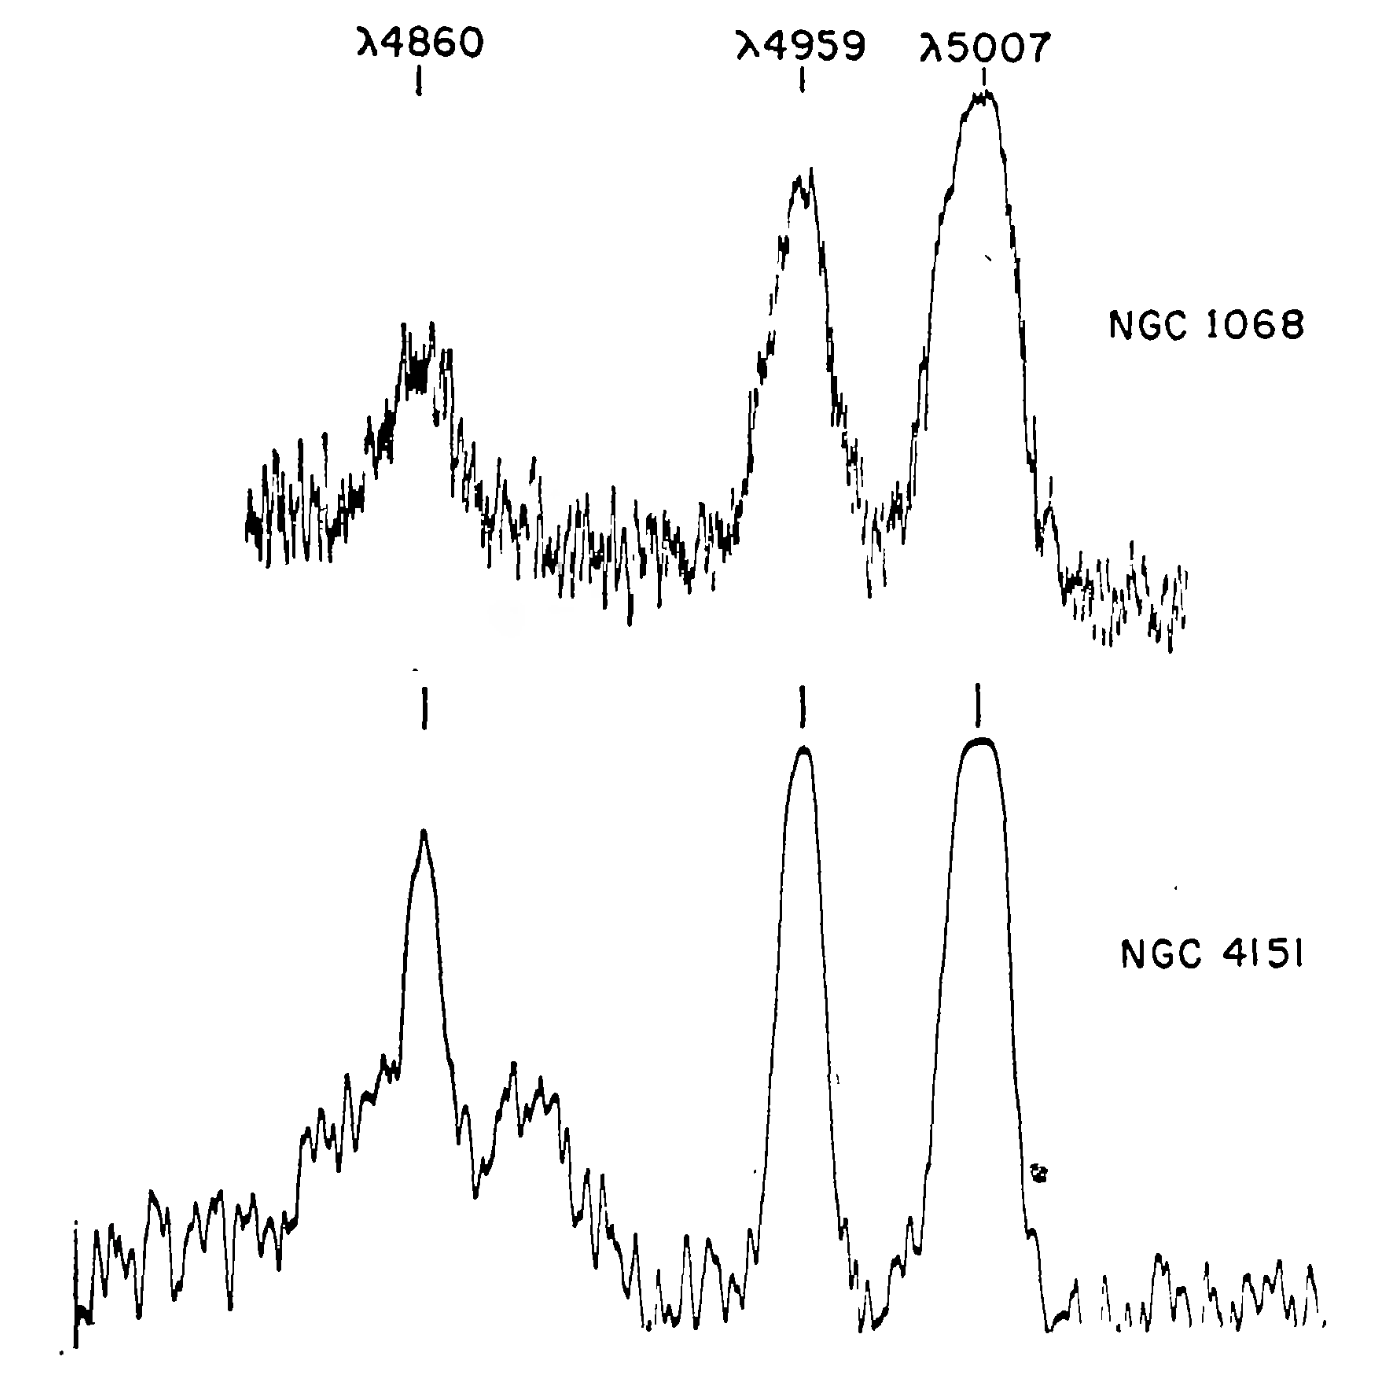
\includegraphics{figures/introduction/seyfert1943_spectra.png}
    \caption[Emission-line profiles for NGC\;1068 and NGC\;4151 as presented by \citet{Seyfert1943}.]{H$\beta$ and [OIII]$\lambda\lambda4959,5007$ emission line profiles for NGC\;1068 and NGC\;4151, as presented by \citet{Seyfert1943}. A prominent broad component can be seen only in H$\beta$ (a permitted line) in NGC\;4151. \textit{Image credit: Carl Seyfert (\citealt{Seyfert1943}; edited by the present author)}.}
    \label{fig: introduction: historical_context: seyfert1943_spectra}
\end{figure}

\newpage
\subsection{The advent of radio astronomy}
\label{section: introduction: historical_context: radio_astronomy}

While working as an engineer for Bell Telephone Laboratories in the early 1930s, Karl Jansky\footnote{A detailed account of Jansky's work and the history of radio astronomy, based on publications and private communications, is given by \citet{Kellerman2023}, from which relevant details are given in this section.} investigated sources of noise affecting shortwave ($\lambda$\;\textless\;100\;m; $\nu$\;\textgreater\;3\;MHz), long-distance telephone communications. Starting in 1930, Jansky used a directional antenna that could rotate fully in azimuth, allowing him to determine the directions of different sources of noise. Working at a wavelength of 14.5\;m (20.5\;MHz), he detected transmissions from stations in South America and England, in addition to noise generated by both distant and local thunderstorms. Although the noise from the storms was dominant, Jansky was also able to detect another source that did not correspond to known weather events. The apparent direction of the peak of this noise changed with the time of day and year, and its source was unclear until Jansky consulted his friend Melvin Skellet, a PhD student in astronomy, who recognised that its position corresponded to the Galactic plane of the Milky Way.

Although Jansky had --- for the first time in history --- observed the night sky at a different wavelength to the optical, his results attracted little attention. A later press release led to wider recognition, after which he published papers on his so-called `star noise' in \textit{the Proceedings of the IRE} \citep{Jansky1933b} and \textit{Nature} \citep{Jansky1933a}. However, his responsibilities at Bell Laboratories took precedence, and he was unable to comprehensively investigate cosmic radio emission further.

While the astronomical community took effectively no notice of Jansky's work, other radio engineers did. Perhaps most notable of these was Grote Reber, who built a steerable parabolic dish dedicated to studying cosmic radio emission and mapped the sky at various frequencies. Reber's radio maps showed not only diffuse emission along the Galactic plane, but also several maxima \citep{Reber1944}, including one in the constellation Cygnus (the maximum in which would later be labelled Cygnus\;A).

Radio astronomy flourished after the conclusion of the Second World War as a result of an abundance of experienced radar technicians, radio experts, and former military equipment. Of particular interest to the early radio astronomy community was Cygnus\;A, which was identified as a discrete source during the war \citep{Hey1946}. Subsequent sea-cliff interferometric observations by J.G. Bolton \& G.J. Stanley identified other discrete sources in addition to Cygnus\;A (see \citealt{Kellerman2023}, Chapter 3), and interest quickly grew in these `radio stars'. However, their natures were poorly understood, and the low astrometric precision of early radio observations made the identification of optical counterparts difficult.

Despite this, through the use of sea-cliff interferometry, \citet{Bolton1949} were able to achieve sufficiently precise radio-source positions to identify the optical counterparts of three of them: Taurus A was identified with the Crab Nebula (M1); Virgo A was identified with M87 (a large elliptical galaxy with an elongated structure\footnote{The narrow, elongated structure in M87 was first identified at optical wavelengths by \citet{Curtis1918}, who noted "a curious straight ray" associated with the object, which is now recognised as an AGN jet. For the definition of AGN jets used in this thesis, see the \hyperref[chapter: definitions]{Definitions} section.}), and Centaurus A was identified with the elliptical galaxy NGC\;5128. Further accurate radio-interferometric positions by \citet{Smith1951} allowed \citet{Baade1954} to identify the optical component of Cygnus\;A: a galaxy at a redshift of $z=0.056$ presenting forbidden lines (such as [OIII], [OII], [NeV]) and H$\alpha$ with relatively broad line widths ($\sim$400\;km\;s$^{-1}$), similar to Seyfert nuclei. It thus became clear that many discrete radio sources were extragalactic, and the correspondingly large distances implied unprecedented luminosities. By the end of the 1950s, it was appreciated that `radio galaxies' such as these should be detectable up to high redshifts --- this provoked great interest among astronomers, since source number counts at the corresponding distances could discriminate between competing cosmological models.

Also at this time, spectroscopic follow-up observations of the radio source 3C\;48 --- a stellar-like object with faint nebulosity --- revealed broad emission lines that did not correspond to any known atomic or ionic transition, and optical imaging showed excess ultraviolet (UV)-emission (see discussion in \citealt{Shields1999}). Similar broad lines and UV-excesses were later associated with other radio sources, which were labelled Quasi-Stellar Sources (QSS) or Quasi-Stellar Objects (QSO); eventually, this terminology was shortened to `quasars'\footnote{The term `quasar' was first used by \citet{Chiu1964}, however, it was first defined in scientific literature --- along with the terms `QSO' and `QSS` --- by \citet{Schmidt1970}, who defined them as being ``objects of starlike appearance ... that exhibit redshifts much larger than those of ordinary stars''. For the definition of the term `Quasar' used throughout this thesis, see the \hyperref[chapter: definitions]{Definitions} section.}. The true nature of these objects was discovered when Maarten Schmidt performed optical follow-up observations of the radio source 3C\;273, an accurate position and angular extent for which had been recently established by \citet{Hazard1963} during a lunar occultation. In optical imaging, 3C\;273 appeared as a 13th-magnitude star, while the spectra revealed that the `star' had broad lines at unfamiliar wavelengths, similar to those identified with 3C\;48 previously. Noting a series of four emission lines of decreasing flux, Schmidt realised that the lines could be explained as the Balmer recombination series of hydrogen if they were redshifted by $z=0.16$. This in turn allowed for the identification of the UV emission line Mg\;II\;$\lambda2798$ in both 3C\;273 and 3C\;48; the redshift of the latter was determined to be $z=0.37$. These results were published in adjacent papers in the journal \textit{Nature} \citep{Hazard1963, Schmidt1963, Oke1963, Greenstein1963}, and quasars were thus identified as active galaxies with spectra similar to those seen in Seyfert nuclei, albeit with higher luminosities.

However, it was not clear what the mechanism responsible for the extreme luminosities of quasars and Seyfert galaxies was, nor how it could be responsible for the observed spectra. An early attempt to understand this was made by \citet{Woltjer1959} who, based on the observed fraction of spiral galaxies that have Seyfert-like nuclei, the fact that the nuclei are spatially-unresolved in imaging, and a virial argument involving observed line widths, estimated that the high luminosities of observed Seyfert nuclei were generated by a 10$^{8-9}$\;M$_\odot$ object in a compact volume (\textless\;100\;pc$^{-3}$). Five years later, \citet{Salpeter1964} and \citet{Zeldovich1964} proposed that this could be understood as accretion onto supermassive black holes (SMBHs), as a non-rotating SMBH could release 0.057c$^2$ of energy per unit mass: sufficient to power the observed luminosities of quasars and Seyfert nuclei.

This argument was popularised by \citet{LyndenBell1969}, who postulated that `dead quasars' (i.e. quiescent SMBHs) should be common in the nuclei of all galaxies, given the energy output of quasars seen at higher redshifts (corresponding to earlier cosmological times). Moreover, \citet{LyndenBell1969} determined that the emission expected from accretion disks around active SMBHs could photoionise gas in galactic nuclei, leading to the spectra observed in quasars. Therefore, by the late 1960s, not only were the central AGN-engines of active galaxies (e.g. Seyferts and quasars) beginning to be understood, but it was appreciated that their unprecedented luminosities may impact their host galaxies, motivating studies in the following decades that sought to understand the nature of this impact.

\subsection{Narrow-line studies of active galaxies}
\label{section: introduction: historical_context: nlr_studies}

\subsubsection{The connection between ionised gas and radio structures}
\label{section: introduction: historical_context: nlr_studies: early_outflows}

An important characteristic of active galaxies, identified since the earliest spectroscopic observations (e.g. \citealt{Slipher1917, Campbell1918, Seyfert1943}; Figure \ref{fig: introduction: historical_context: seyfert1943_spectra}), is the presence of narrow (full width at half maximum (FWHM)\;\textless\;1000\;km\;s$^{-1}$) and broad (FWHM\;\textgreater\;1000\;km\;s$^{-1}$) emission-line profiles. Due to their associated velocities being a significant fraction of the speed of light, the broad lines received much attention in studies of active galaxies, while the narrow lines were of less interest (see discussion in \citealt{Krolik1984}). 

While \citet{Seyfert1943} recognised that narrow line broadening (100\;\textless\;FWHM\;\textless\;1000\newline km\;s$^{-1}$) was due to the Doppler shifting of lines within the objects, the physical implication of this was first considered by \citet{Burbidge1958}, who noted that the line widths corresponded to velocities that were much higher than the galactic escape velocities and therefore ``the interstellar gas in the nuclear regions must be constantly escaping from the galaxy as a whole". This was subsequently supported by a study of the inner regions ($r$\;\textless\;2\;kpc) of the archetypal Seyfert galaxy NGC\;1068, which showed that the observed line widths implied velocities that are more than three times that of the escape velocity on these scales \citep{Burbidge1959}. 

Higher-spatial-resolution optical spectroscopy at different spatial positions and position angles (PAs) allowed for the identification of discrete clouds responsible for the observed line broadening in active galaxies (particularly NGC\;1068 and NGC\;4151: e.g. \citealt{Merle1968, Anderson1970, Glaspey1976}). These clouds were found to have velocity shifts in the range 100\;\textless\;$v$\;\textless\;1000\;km\;s$^{-1}$: higher than the escape velocity at their radii ($r$\;\textless\;$500$\;pc). This supported the idea of an `expansion' of gas away from the nuclei, an interpretation that was refined by \citet{Heckman1981}, who argued that observed asymmetries in the narrow-line profiles in a sample of 36 active galaxies were due to AGN-driven radial outflows of gas (see also \citealt{Grandi1977} and \citealt{Heckman1983}).

Simultaneously, studies throughout the 1970s began to investigate the physical conditions (including temperatures, densities, reddenings, and compositions) of the narrow-line-emitting gas, with a particular focus on determining how it is ionised. The prevailing candidate ionisation mechanisms were photoionisation via radiation emitted by AGN accretion disks (e.g. \citealt{MacAlpine1972, Baldwin1975, Shields1975, OsterbrockKoski1976, Ferland1979}) and astrophysical shock-waves propagating through the interstellar mediums (ISMs) of the host galaxies (e.g. \citealt{Cox1972, Koski1976, Fosbury1978, Penston1978}). Combined with the presence of outflowing gas, this indicated that AGN were having a significant impact on the central regions of galaxies.

Also in this time period, new radio observatories (such as the Westerbork Synthesis Telescope, the National Radio Astronomy Observatory 300-foot radio telescope, and the Mullard Radio Astronomy Observatory) were used to perform both large surveys of the local AGN population and detailed studies of individual objects. The radio surveys performed with these facilities found that galaxies with Seyfert nuclei had radio luminosities that were higher than those of normal (quiescent) spiral galaxies, but less than those of the `radio galaxies' discovered in the decades prior \citep{vanderKruit1973, Sramek1975}. The advent of higher-spatial-resolution radio observations in the 1980s, permitted by new facilities such as the Very Large Array (VLA) and Multi-Element Radio Linked Interferometer Network (MERLIN), revealed that the radio morphologies of Seyfert galaxies often consisted of two or more components, connected by fainter emission on arcsecond (kiloparsec) scales (e.g. \citealt{Wilson1980, Wilson1982, Pedlar1983, Pedlar1984, Ulvestad1984}; Figure\;\ref{fig: introduction: historical_context: nlr_studies: wilson1982_ngc1068_15ghz}) --- similar to what had previously been identified on much larger scales in powerful radio galaxies such as Cygnus A \citep{Jennison1959}. These double and triple radio structures were interpreted as synchrotron emission produced by AGN jets \citep{Wilson1980}: fast (up to tenths of the speed of light), collimated streams of plasma that are launched from AGN accretion disks along the spin axis of the central SMBH (see \citealt{Rees1984} for a contemporary review). In this scenario for Seyfert galaxies, the radio emission observed at the position of the optical nucleus (the core) originates from the central AGN engine, while the extended radio component(s) (the lobes) represent the termination point of the jet and/or prominent interactions of the jet with the ISM of the host galaxy \citep{Wilson1980, Sanders1984}.

\begin{figure}[!t]
    \centering
    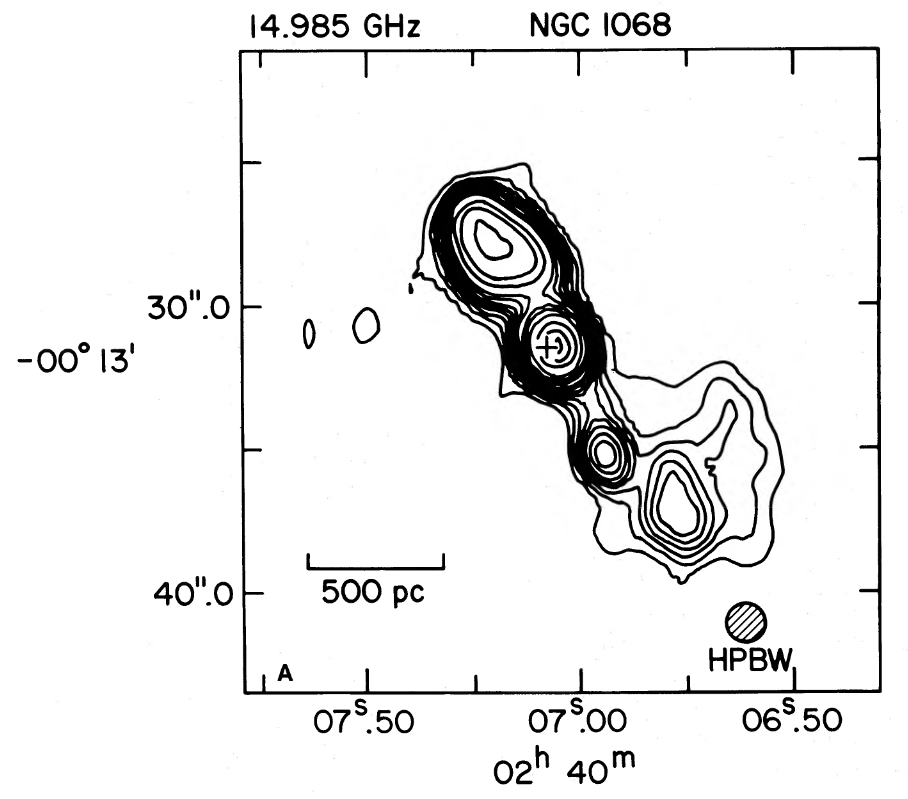
\includegraphics[width=0.8\linewidth, trim={0 0 -3cm 0}, clip]{figures/introduction/ulvestad1982_ngc1068_15ghz.png}
    \caption[14.985\;GHz radio map of the inner kiloparsecs of the Seyfert galaxy NGC\;1068 (as presented by \citealt{Wilson1982}), showing a linear radio structure.]{14.985\;GHz map of the inner kiloparsecs of the Seyfert galaxy NGC\;1068, showing a linear, triple radio structure consisting of a core (coincident with the optical nucleus, marked by the cross) and two radio lobes. The contours are 1, 2, 3, 4, 5, 6, 8, 10, 15, 20, 30, 50, 70 and 90\;per\;cent of 192.5\;mJy\;beam$^{-1}$. \textit{Image credit: \citet{Wilson1982}}.}
    \label{fig: introduction: historical_context: nlr_studies: wilson1982_ngc1068_15ghz}
\end{figure}

Concurrently, multi-wavelength studies utilising both optical and radio observations discovered empirical correlations between the radio and narrow-line properties of Seyfert galaxies, notably between 1.4\;GHz (21\;cm) and [OIII] luminosity \citep{deBruyn1978}, and 1.4\;GHz luminosity and [OIII] line width \citep{Wilson1980}. Furthermore, high-spatial-resolution observations revealed that in many cases, the major axes of linear radio structures and optical narrow-line emission were aligned (\citealt{Ulvestad1981}; see Table 2 in \citealt{Wilson1985}). This implied a physical relationship between the radio- and narrow-line-emitting material; although the nature of this connection was not clear, suggestions were made that plasma jets were interacting with the ISMs of host galaxies, ionising the gas and accelerating outflows (see Section 3 of \citealt{Wilson1985}).

The relationship between narrow-line-emitting gas and radio structures was first directly investigated by \citet{Whittle1988}, who used spatially-resolved spectroscopic observations of 10 Seyfert galaxies that presented double or triple linear radio structures. It was found that, not only was the [OIII] and H$\beta$ line emission strongly spatially associated with the radio structures, but their line profiles were particularly complex at the locations of bright radio emission. The derived narrow-line velocities were high (150\;\textless\;$v$\;\textless\;1000\;km\;s$^{-1}$), with the highest velocities found at the position of the enhanced radio emission. This indicated that the gas was more kinematically disturbed at these locations, and thus that prominent AGN-driven outflows are associated with radio structures on kiloparsec-scales.

\subsubsection{The unified scheme of AGN and ionisation cones}
\label{section: introduction: historical_context: nlr_studies: unified scheme}

As seen in the spectra presented by \citet{Seyfert1943} (Figure \ref{fig: introduction: historical_context: seyfert1943_spectra}), there exists a dichotomy in AGN regarding the widths of permitted and narrow lines. Some objects, termed Seyfert\;1s (Sey\;1, later generalised to Type 1 AGN) present narrow forbidden lines and broad permitted lines, while others (Seyfert 2, or Sey\;2; generalised to Type 2 AGN) show narrow forbidden and permitted lines (see \citealt{Khachikian1971}). The underlying mechanism responsible for this was confirmed by \citet{Antonucci1985}, who used spectropolarimetric measurements of the Sey\;2 galaxy NGC\;1068 to demonstrate the presence of polarised broad permitted lines. This indicated that the source of the broad permitted lines --- known as the broad line region (BLR) --- also existed in Type 2 AGN, but was obscured by a torus-like structure (which may be clumpy: \citealt{Nenkova2002, Nenkova2008}; see Section\;2.3 of \citealt{Netzer2015}), and confirmed that Type 1 and Type 2 AGN were intrinsically the same phenomenon, only viewed at different angles with respect to the observer (Figure\;\ref{fig: introduction: historical_context: nlr_studies: unified_scheme}).

\begin{figure}[!ht]
    \centering
    \includegraphics[width=\linewidth]{figures/introduction/unified_scheme.png}
    \caption[Schematic of the unified scheme of AGN.]{Schematic of the unified scheme of AGN. \textbf{The central supermassive black hole (SMBH; $r\sim10$--100\;AU), accretion disk ($r\sim1000$--10,000\;AU), jet, and obscuring torus ($r\sim0.1$--10\;pc) are labelled with solid black arrows; the locations of the broad line region (BLR; $r\sim100$--1000\;AU) and narrow line region (NLR; $r\sim0.1$--10\;kpc) are also labelled.} The dashed arrows show the lines of sight that result in an AGN being observed as Type\:1 or Type\:2. Not to scale.}
    \label{fig: introduction: historical_context: nlr_studies: unified_scheme}
\end{figure}

Optical observations of the narrow line regions (NLRs; kiloparsec-scale regions of narrow-line emission) of Seyfert galaxies in the late 1980s and early 1990s revealed interesting morphologies: the narrow-line-emitting gas appeared to be distributed in conical shapes, the apexes of which corresponded to the position of active nuclei (\citealt{Pogge1988, Pogge1989, Pogge1990, Tadhunter1989, Cecil1990, Miller1990, Evans1991}). In many cases, there was evidence of two cones lying in opposite directions along the same axis --- known as a bicone --- and in almost all cases the (bi)cones were aligned with the radio axes of the objects.

The launch of the Hubble Space Telescope (HST) in 1990\footnote{A grounding error in the HST's primary mirror produced significant spherical aberration in observations until it was fixed during a service mission in 1993. Despite this, the telescope was still scientifically useful for studies of nearby AGN during this period.} allowed optical studies of unprecedented spatial resolution, which showed that the NLR quiescent and outflowing gas structures were much more complex than indicated by earlier observations. While many authors argued, based on spatially-resolved gas kinematics and conditions, that outflows in Seyfert galaxies are driven via shocks induced in the ISM by radio jets (e.g. \citealt{Taylor1992, Bower1995, Capetti1995a, Capetti1995b, Axon1998}), others argued that radiation pressure from accretion disks also contributed to outflow acceleration (and is perhaps the dominant driving mechanism). In the latter scenario, this driving is done either by fast ($\sim$0.1\;$c$) winds launched close to the nucleus (called nuclear winds) that shock the cold ISM on larger scales and accelerate outflows (e.g. \citealt{Cecil1990}), or by direct radiation pressure acting on the NLR gas (e.g. \citealt{Crenshaw2000_N1068, Crenshaw2000_N4151, Kaiser2000}).

\subsection{AGN-driven outflows and galaxy evolution}
\label{section: introduction: historical_context: galaxy evolution}

Early studies which interpreted complex narrow-line profiles in Seyfert galaxies as being due to `expansion' (e.g. \citealt{Walker1968, Anderson1970, Glaspey1976}), and later outflows of gas (e.g. \citealt{Grandi1977, Heckman1981}), indicated that AGN were having an impact on the central kiloparsecs of galaxies. However, the first recognition that AGN-driven outflows may play an important role in how galaxies evolve was by \citet{Sanders1988}. Noting that ultra luminous infrared galaxies (ULIRGs; $L_\mathrm{IR}$\;\textgreater\;$10^{12}$\;L$_\mathrm{\odot}$: \citealt{Sanders1988, Sanders1996}) present merger-like morphologies and host bright nuclei, \citet{Sanders1988} proposed that these objects contained obscured quasar-like nuclei which drive high-mass gas outflows that remove or destroy the obscuring dust. In this scenario, ULIRGs transition into quasars, forming an evolutionary sequence.

However, the main impetus for studying AGN-driven outflows came in the mid-1990s, when empirical scaling relations between SMBH masses and host-galaxy bulge properties (luminosity, velocity dispersion, and stellar mass; Figure\;\ref{fig: introduction: historical_context: galaxy_evolution: ferrarese2000_mbh_vdisp}) were discovered \citep{Kormendy1995, Magorrian1998, Gebhardt2000, Ferrarese2000}. The form of these correlations could be readily explained by SMBHs and galactic bulges accreting the same material (i.e. gas inflows to the centres of galaxies), however, this could not explain their tightness --- an additional mechanism was thought to be required. Outflows driven by AGN were first invoked to be this additional mechanism by \citet{Silk1998}, who created an analytic model that required a small fraction of AGN luminosity to couple to the ISMs of host galaxies, driving galaxy-wide outflows which set the tightness of the observed scaling relations. AGN-driven outflows subsequently became the basis of further analytic models that could explain the empirical SMBH-bulge scaling relations (e.g. \citealt{Fabian1999, King2003}).

\begin{figure}
    \centering
    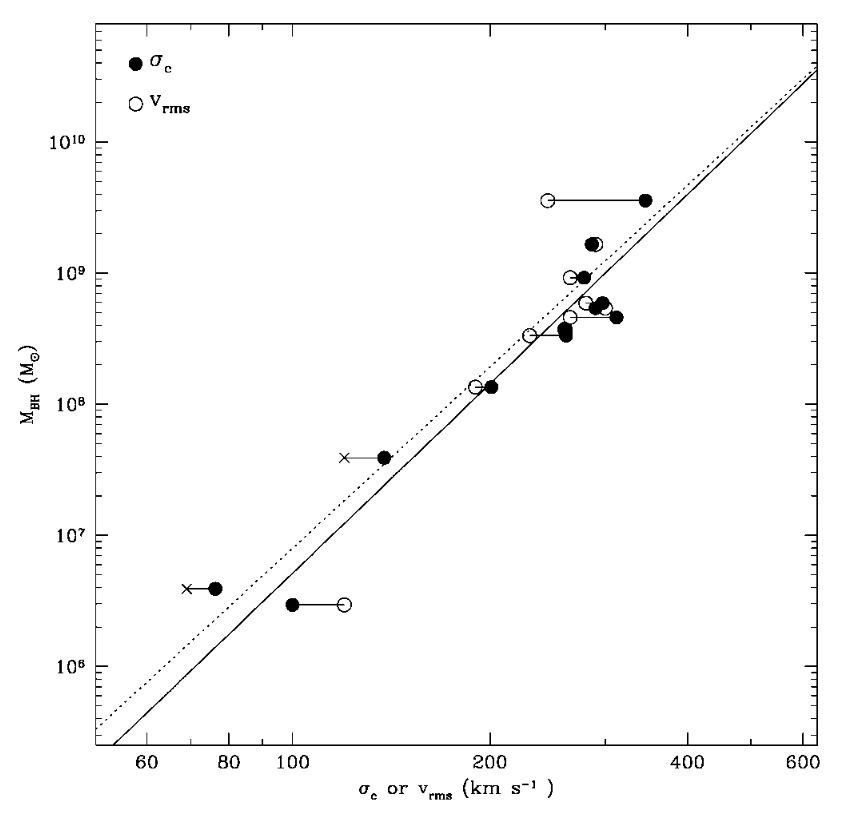
\includegraphics[width=0.9\linewidth]{figures/introduction/ferrarese2000_mbh_vdisp.png}
    \caption[Empirical scaling relation between supermassive black hole mass and galactic bulge stellar velocity dispersion, presented by \citet{Ferrarese2000}.]{Empirical scaling relation between supermassive black hole mass and stellar velocity dispersion ($\sigma_c$: filled circles) or root-mean-square (rms) velocity ($v_{rms}$: hollow circles; crosses represent lower limits) as presented by \citet{Ferrarese2000}. The dashed and solid lines represent the best linear fits. \textit{Image credit: \citet{Ferrarese2000}}.}
    \label{fig: introduction: historical_context: galaxy_evolution: ferrarese2000_mbh_vdisp}
\end{figure}

In addition, AGN also began to be invoked to explain several other observed features of galaxies and their environments (see \citealt{Cattaneo2009} for a contemporary review), such as AGN jets heating and preventing the cooling of highly-ionised, hot X-ray-emitting gas that is observed in and around galaxy clusters \citep{McNamara2007, Gaspari2013} and the luminosity function of the local galaxy population \citep{Benson2003}. The collective impact that AGN are thought to have on their host galaxies is referred to as AGN feedback, which is now a crucial component of models of galaxy evolution (including detailed hydrodynamical simulations: e.g. \citealt{DiMatteo2005, Springel2005, Hopkins2010}; and cosmological simulations: e.g. \citealt{Schaye2015, Dave2019, Zinger2020}). While AGN-driven outflows are thought to be required to explain SMBH-bulge scaling relations, they are also now commonly considered to be an important aspect of AGN feedback in general, and therefore have become the focus of an increasing number of studies over the past thirty years (Figure\;\ref{fig: introduction: historical_context: galaxy_evolution: harrison2018_abstracts}).

\begin{figure}
    \centering
    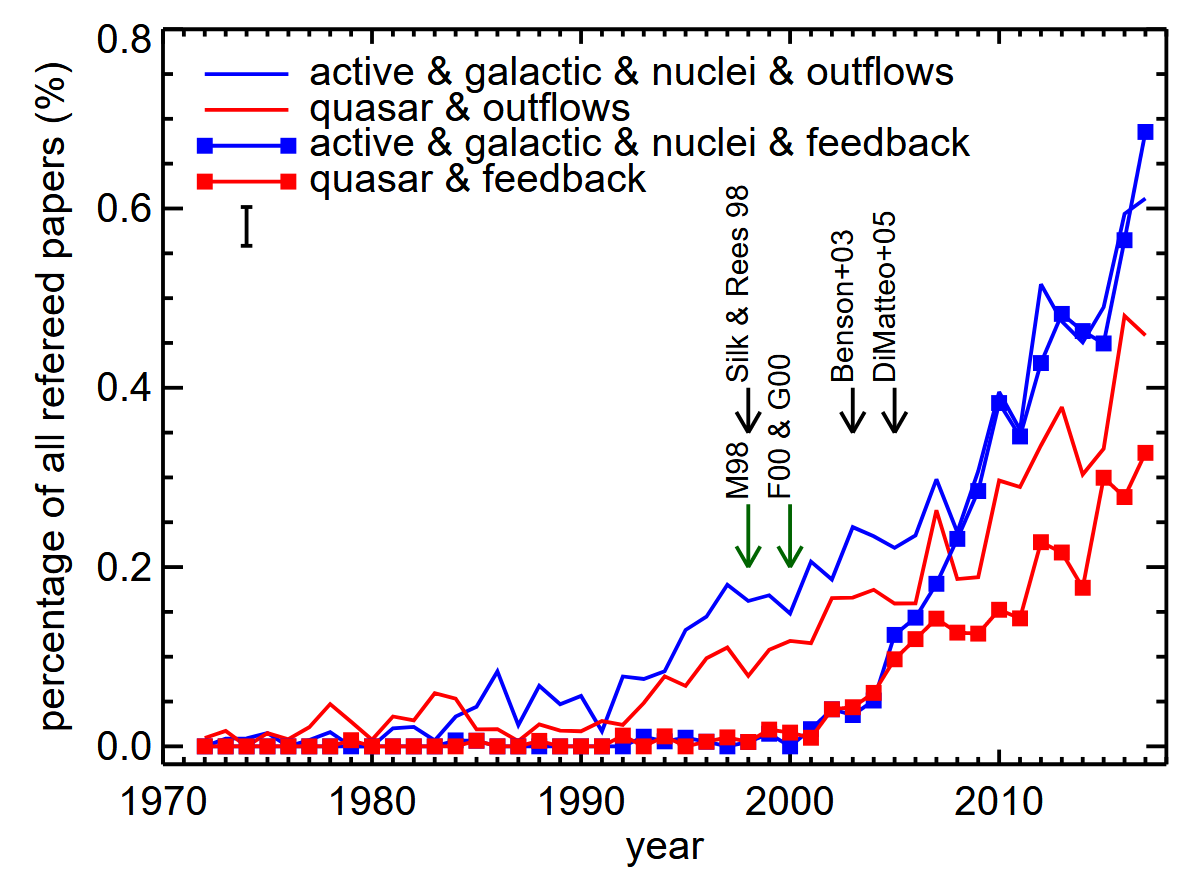
\includegraphics[width=0.85\linewidth]{figures/introduction/harrison2018_abstracts.png}
    \caption[Cumulative number of published AGN-driven outflow studies since the early 1970s, taken from \citet{Harrison2018}.]{Percentage of peer-reviewed publications from 1970 to 2018 that contain the keywords given in the legend (top left) in their abstracts. The publication dates of key studies (M98: \citealt{Magorrian1998}; F00: \citealt{Ferrarese2000}; G00: \citealt{Gebhardt2000}; \citealt{Benson2003, DiMatteo2005}) which produced a significant increase in interest of AGN-driven outflows are marked with vertical arrows. \textit{Image credit: \citealt{Harrison2018}.}}
    \label{fig: introduction: historical_context: galaxy_evolution: harrison2018_abstracts}
\end{figure}

\newpage
\section{AGN-driven outflows}
\label{section: introduction: outflows: introduction}

The first hydrodynamical simulation of the impact of AGN-driven outflows on galaxy evolution was performed by \citet{DiMatteo2005}, who modelled a major galaxy merger with SMBHs as sink particles. These SMBHs injected thermal energy ($E_\mathrm{feed}$) into the ISM of the merger as
\begin{equation}
    E_\mathrm{feed}=\epsilon_\mathrm{f}\eta_\mathrm{r}\dot{M}_\mathrm{BH}c^2
    \label{eq: introduction: outflows: introduction: dimatteo2005_efeed}
\end{equation}
where $\eta_\mathrm{r}$ is the radiative efficiency of the SMBH accretion disk, $\dot{M}_\mathrm{BH}$ is the accretion rate onto the SMBH, and $c$ is the speed of light. Here, $\epsilon_\mathrm{f}$ is a free parameter known as the coupling efficiency (or coupling factor): the fraction of radiation coupled to the ISM of the host galaxy. In this model, the coupling of radiation to the ISM launches galaxy-wide ($r$\;\textgreater\;5\;kpc) outflows, heating and expelling gas needed to form stars, hence suppressing star formation. 

The coupling efficiency in the \citet{DiMatteo2005} simulation was set to the value required ($\epsilon_\mathrm{f}=0.05=5$\;per\;cent) to reproduce the normalisation of the observed relation between SMBH mass and bulge stellar velocity dispersion (known as the $M$-$\sigma$ relation; Figure\;\ref{fig: introduction: historical_context: galaxy_evolution: ferrarese2000_mbh_vdisp}). Subsequent theoretical work also invoked galaxy-wide, AGN-driven outflows, with each setting a different value of this free parameter to reproduce the normalisation of empirical relations (typically 0.5\;\textless\;$\epsilon_\mathrm{f}$\;\textless\;10\;per\;cent: \citealt{Springel2005,Hopkins2010}). In the 2010s, large-scale cosmological simulations incorporated a similar approach to their AGN-feedback prescriptions, requiring a fraction of energy produced by accreting SMBHs in galactic centres to be coupled to host galaxies (e.g. $\epsilon_\mathrm{f}=0.15=15$\;per\;cent for EAGLE and Horizon-AGN: \citealt{Schaye2015, Dubois2016}), restricting star formation and therefore reproducing the observed properties of the local galaxy population. 

Motivated by these theoretical models, observational studies of AGN-driven outflows often interpret the coupling efficiency as being the ratio between outflow kinetic power ($\dot{E}_\mathrm{kin}$: kinetic energy per unit time) and AGN bolometric luminosity ($L_\mathrm{bol}$):

\begin{equation}
    \epsilon_\mathrm{f}=\frac{\dot{E}_\mathrm{kin}}{L_\mathrm{bol}}.
    \label{eq: introduction: outflows: introduction: e_f}
\end{equation}

Therefore, in attempts to verify the models --- and hence the role of AGN-driven outflows in galaxy evolution --- a large number of studies in the past twenty-five years have focused on measuring coupling efficiencies in this way and comparing them to the free parameter set by models. Many observational studies have derived coupling efficiencies that fall in the range required by theoretical work (0.5\;\textless\;$\epsilon_\mathrm{f}$\;\textless\;10\;per\;cent: e.g. \citealt{Liu2013, Harrison2014, Cicone2014, Fiore2017}), however, there are several major sources of uncertainty associated with this approach which render its validity unclear.

Principally, observationally-derived outflow kinetic powers are not well constrained: due to many factors, commonly-determined values may be incorrect by several orders of magnitude. Furthermore, the validity of direct comparisons to theoretical models using coupling efficiencies is unclear, as is the robustness of interpretations that are made from such comparisons regarding the impacts of AGN-driven outflows on host galaxies (see discussion in \citealt{Harrison2018}); largely, this is because it is unclear exactly \textit{how} AGN accelerate outflows. In the following sections, I review and explain these uncertainties.

\subsection{Uncertainties regarding outflow energetics}
\label{section: introduction: outflows: energetics}

\subsubsection{The multi-phase nature of outflows}
\label{section: introduction: outflows: energetics: multi-phase}

The ISM is observed in a range of gas phases: regimes of different temperatures and conditions, ranging from hot and highly-ionised to cold and molecular. Similarly, AGN-driven outflows have been observed in multiple phases, corresponding to distinct temperatures and compositions of the emitting gas (see \citealt{Cicone2018} for a review). Different phases are observed with tracers at different wavelengths --- Table\;\ref{tab: introduction: outflows: energetics: multi-phase: outflow_phases} presents the phases considered in this thesis, and examples of their observational tracers.

\begin{table}[!t]
    \vspace*{-1cm}
    \centering
    \centerline{
    {\renewcommand{\arraystretch}{4}
    \begin{tabular}{ccc}
        Phase & Temperature range & Observational tracers \\
        \hline
        \parbox{4cm}{\hspace*{\fill} Highly ionised \hspace*{\fill}} & \textgreater\;$10^6$\;K & \parbox{8cm}{Hard X-ray ($E_\gamma$\;\textgreater\;6\;keV) absorption lines \\ \hspace*{\fill} (e.g. Fe\;XXV, Fe\;XXVI); \hspace*{\fill} \\ \hspace*{\fill} X-ray continuum \hspace*{\fill}} \\
        Warm ionised & 10,000--30,000\;K & \parbox{8cm}{\hspace*{\fill} UV, optical, near-infrared, and \hspace*{\fill} \\ \hspace*{\fill} mid-infrared emission lines \hspace*{\fill} \\ \hspace*{\fill} (e.g. [OIII]$\lambda\lambda4959,5007$, H$\beta$, Pa$\beta$, \hspace*{\fill} \\ \hspace*{\fill} [SII]$\lambda\lambda6717,6731$, HeI, [O IV]\;25.9\;$\mu$m) \hspace*{\fill}} \\
        Warm molecular & $\sim2000$\;K & \parbox{8cm}{\hspace*{\fill} Near-infrared roto-vibrational \hspace*{\fill} \\ \hspace*{\fill} emission lines of H$_2$ \hspace*{\fill} \\ \hspace*{\fill} (e.g. H$_2$(1--0)S(1)\;2.212\;$\mu$m, \hspace*{\fill} \newline \hspace*{\fill} H$_2$(2--1)S(1)\;2.247\;$\mu$m) \hspace*{\fill}} \\
        Neutral atomic & 100--2000\;K & \parbox{8cm}{\hspace*{\fill} Radio emission lines  (e.g. HI\;21\;cm line), \hspace*{\fill} \\ \hspace*{\fill} optical NaID absorption lines \hspace*{\fill} \\ \hspace*{\fill} (NaID$\lambda\lambda$5890,5896) \hspace*{\fill}} \\
        Cold molecular & 10--300\;K & \parbox{8cm}{\hspace*{\fill} Radio/sub-mm emission \& absorption lines \hspace*{\fill} \\ \hspace*{\fill} (e.g. CO(1--0), CO(2--1), HCN, OH) \hspace*{\fill}} \\
    \end{tabular}
    }
    }
    \caption[The gas phases of AGN-driven outflows that are considered in this thesis.]{The gas phases of AGN-driven outflows that are considered in this thesis, their approximate temperatures, and examples of their observational tracers (wavelength regime and example spectral features).}
    \label{tab: introduction: outflows: energetics: multi-phase: outflow_phases}
\end{table}

Since the majority of studies use observations of only one phase (commonly the warm-ionised gas, due to it producing prominent optical emission lines), it is not clear which outflow phase is dominant in terms of mass and kinetic power. In a relatively small number of active galaxies, the properties of outflows in multiple phases have been quantified (e.g. \citealt{Morganti2005, Holt2011, Tadhunter2014, Riffel2015, Feruglio2015, Morganti2016, Finlez2018, Fluetsch2019}); in some objects, these phases have been seen to be co-spatial and co-kinematic, indicating that they form part of the same outflow (Figure\;\ref{fig: introduction: outflows: energetics: multi-phase: morganti2015_ic5063_multiphase}: \citealt{Tadhunter2014, Morganti2015}).

\begin{figure}[!t]
    \centering
    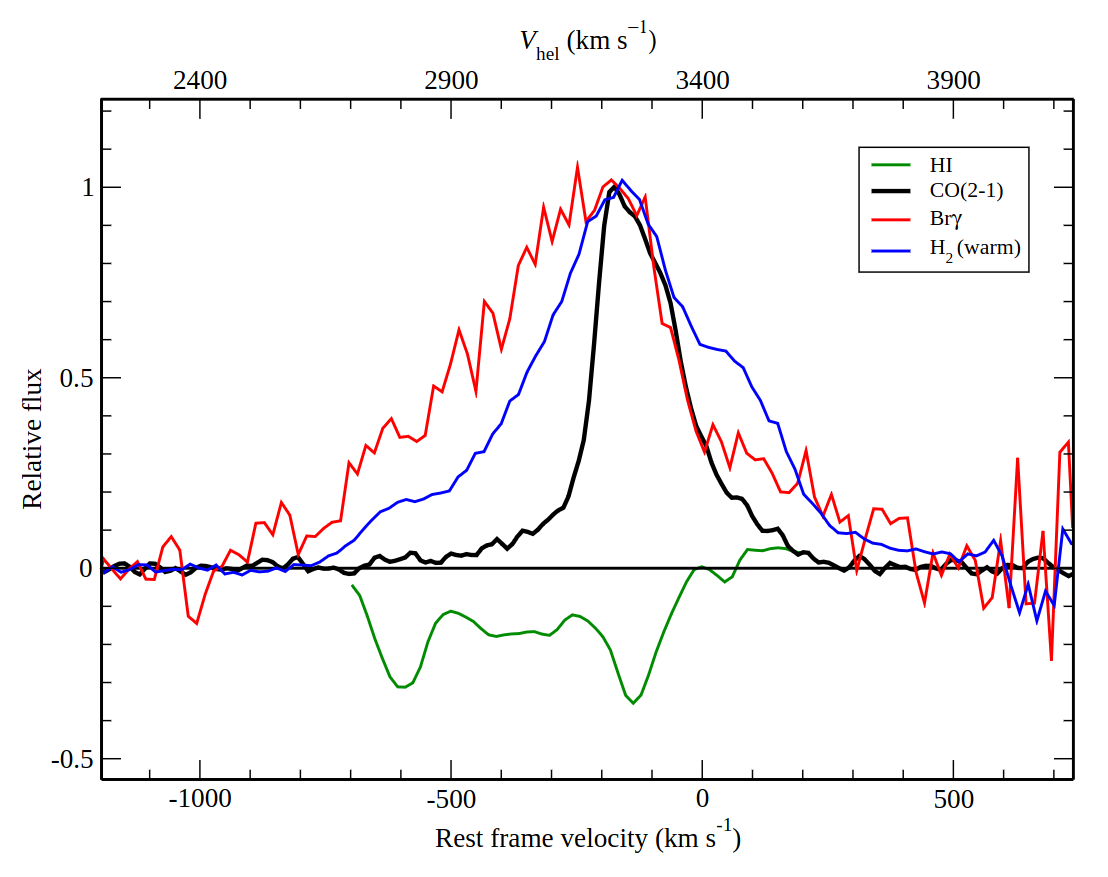
\includegraphics[width=\linewidth]{figures/introduction/morganti2015_ic5063_multiphase.png}
    \caption[Lines arising from different outflow phases in IC\;5063 \citep{Morganti2015}, indicating a co-spatial, co-kinematic multi-phase outflow.]{Line velocity profiles tracing different phases of outflowing gas at the same location in the active galaxy IC\;5063. The red line shows the Br$\gamma$ emission-line profile (warm ionised; \citealt{Tadhunter2014}), the blue line shows the H$_2$(1--0)S(1)\;2.212\;$\mu$m emission-line profile (warm molecular; \citealt{Tadhunter2014}), the green line shows the HI 21\;cm absorption-line profile (neutral atomic; \citealt{Morganti1998}), and the black line shows the CO(2-1) emission-line profile (cold molecular; \citealt{Morganti2015}). Each phase presents outflowing (yet distinct) kinematics, potentially indicating that they are part of the same outflow. \textit{Image credit: \citealt{Morganti2015}}.}
    \label{fig: introduction: outflows: energetics: multi-phase: morganti2015_ic5063_multiphase}
\end{figure}

While some studies present evidence that the cold molecular phase is dominant in terms of mass and kinetic power (i.e. \citealt{Morganti2005, Cicone2014, GarciaBurillo2014}), this has only been determined for a small number of galaxies. Therefore, since the majority of studies only focus on a single phase, it is imperative that the relative masses and powers of multiple phases are comprehensively determined to ensure that \textit{total} outflow kinetic powers are not significantly underestimated.

Moreover, the physical relation between different outflow phases is not understood, nor is it clear how molecular gas can be accelerated to observed outflow velocities ($v$\;\textgreater\;500\;km\;s$^{-1}$) without being dissociated. Understanding this is crucial, as it is required to make quantitative predictions regarding multi-phase outflows. One suggestion is that the various phases in a given gas cloud are accelerated together directly by radiation pressure or cosmic rays \citep{Booth2013, Costa2018, Hopkins2020}, however, in this scenario, it is not clear why the molecules are not photo-disassociated. Other studies propose a solution to this by arguing that the colder, molecular phases are entrained in warmer gas, preventing molecule dissociation \citep{Scannapieco2015, Gaspari2017, Gronke2020}. 

An alternative is that the outflow acceleration mechanism heats the gas to the hot ionised phase ($T$\;\textgreater\;$10^6$\;K), destroying the molecules in the process; as the gas cools post-acceleration, it forms the cooler phases \textit{in-situ}, including the formation of molecules \citep{Wang1995, Silich2003, Tadhunter2014, Zubovas2014, Costa2015, Thompson2016, Richings2021}. A major problem with understanding this scenario is the complexity (and associated difficulty) of modelling molecule formation in the ISM: it is not clear if molecules can form in outflowing-gas conditions on the (highly uncertain) timescales required. In this context, it is interesting to note that recent modelling supports molecule formation and cooling being a sufficiently fast process in outflowing gas \citep{Richings2021}.

Overall, the mass and energy contributions of (and the physical relation between) different outflow phases are not clear --- in order to elucidate this situation, detailed, multi-wavelength observations of multi-phase outflows and their acceleration mechanisms are required.

\subsubsection{Electron densities of warm-ionised outflows}
\label{section: introduction: outflows: energetics: electron_densities}

The most commonly observed outflow phase is warm ionised gas, as many emission lines arising from this phase are present in optical spectra of AGN (Table\;\ref{tab: introduction: outflows: energetics: multi-phase: outflow_phases}). Therefore, many studies that compare outflow kinetic powers to those required by models of galaxy evolution only consider warm-ionised outflow energetics (masses, mass outflow rates, kinetic powers, and coupling efficiencies: e.g. \citealt{Liu2013, Rose2018, Tadhunter2019}). Typically, this is done by first calculating the warm-ionised outflow mass using the measured luminosity of a recombination line of hydrogen ($L(H)$) with
\begin{equation}
    M_\mathrm{out, ion} = \frac{L(H)m_\mathrm{p}}{\alpha^\mathrm{eff}_\mathrm{H}hv_\mathrm{H}n_e},
    \label{eq: introduction: outflows: energetics: mout}
\end{equation}
where $M_\mathrm{out, ion}$ is the mass of the outflowing warm-ionised gas, $m_\mathrm{p}$ is the proton mass, $\alpha^{eff}_{H}$ is the Case B recombination coefficient for the chosen recombination line of hydrogen, $v_\mathrm{H}$ is \textbf{the frequency of the recombination line}, and $n_e$ is the electron density of the emitting gas. This is then used to calculate the mass passing through a given surface area per unit time, known as the mass outflow rate:
\begin{equation}
    \dot{M}_\mathrm{out, ion} = A\cdot\frac{M_\mathrm{out, ion}\;v_\mathrm{out}}{R},
    \label{eq: introduction: outflows: energetics: mout_rate}
\end{equation}
where $v_\mathrm{out}$ is the outflow velocity, $R$ is the outflow radius, and $A$ is a constant that accounts for assumptions regarding outflow geometry and radial density profiles (see Section 2 of \citealt{Veilleux2020}). Finally, the outflow kinetic power is calculated using
\begin{equation}
    \dot{E}_\mathrm{kin, ion} = \frac{1}{2}{\dot{M}_\mathrm{out, ion}(v^2_\mathrm{out} + 3\sigma^2)},
    \label{eq: introduction: outflows: energetics: ekin}
\end{equation}
where $\sigma$ is the velocity dispersion ($\sigma\sim\mathrm{FWHM}$/2.355), which may be interpreted as the range of velocities present \textit{within} a spatially-unresolved region of outflowing gas\textbf{; a multiplicative factor of three is commonly used with this term to account for the velocity dispersion in three dimensions (see \citealt{Rupke2005b}).} Typically, the coupling efficiency (taken to be the ratio of outflow kinetic power to the host AGN bolometric luminosity: Equation\;\ref{eq: introduction: outflows: introduction: e_f}) is then determined and compared to the requirements of theoretical models --- if the observed value is consistent with (or above) these requirements, then the interpretation is often that the outflows have a significant impact on the evolution of the host galaxy.

The largest source of uncertainty when calculating outflow energetics in this way is the electron density of the outflowing gas. Traditionally, the flux ratio of emission lines in a doublet arising from either the SII or OII ion is used (namely [SII](6717/6731) and [OII](3726/3729)): the lines involved in these ratios have similar (but different) critical densities\footnote{The critical density of a transition is defined as the density at which the rate of collisional de-excitation from the upper energy level becomes approximately equal to the collisional excitation rate of electrons to the upper energy level (see Chapter\;5 of \citealt{Osterbrock2006}).}, and so the ratios have a strong dependence on electron density (Figure\;\ref{fig: introduction: outflows: energetics: warm_ionised: sii_ratio})\footnote{The [SII](6717/6731) and [OII](3726/3729) flux ratios also have a dependence on electron temperature. Therefore, when calculating electron densities with these ratios, electron temperatures are either measured using other line ratios (e.g. [OIII](5007+4959)/4363) or assumed to be those typical of the warm ionised phase ($\sim$10,000\;K); see Chapter\;5 of \citet{Osterbrock2006}.}.

\begin{figure}[!ht]
    \centering
    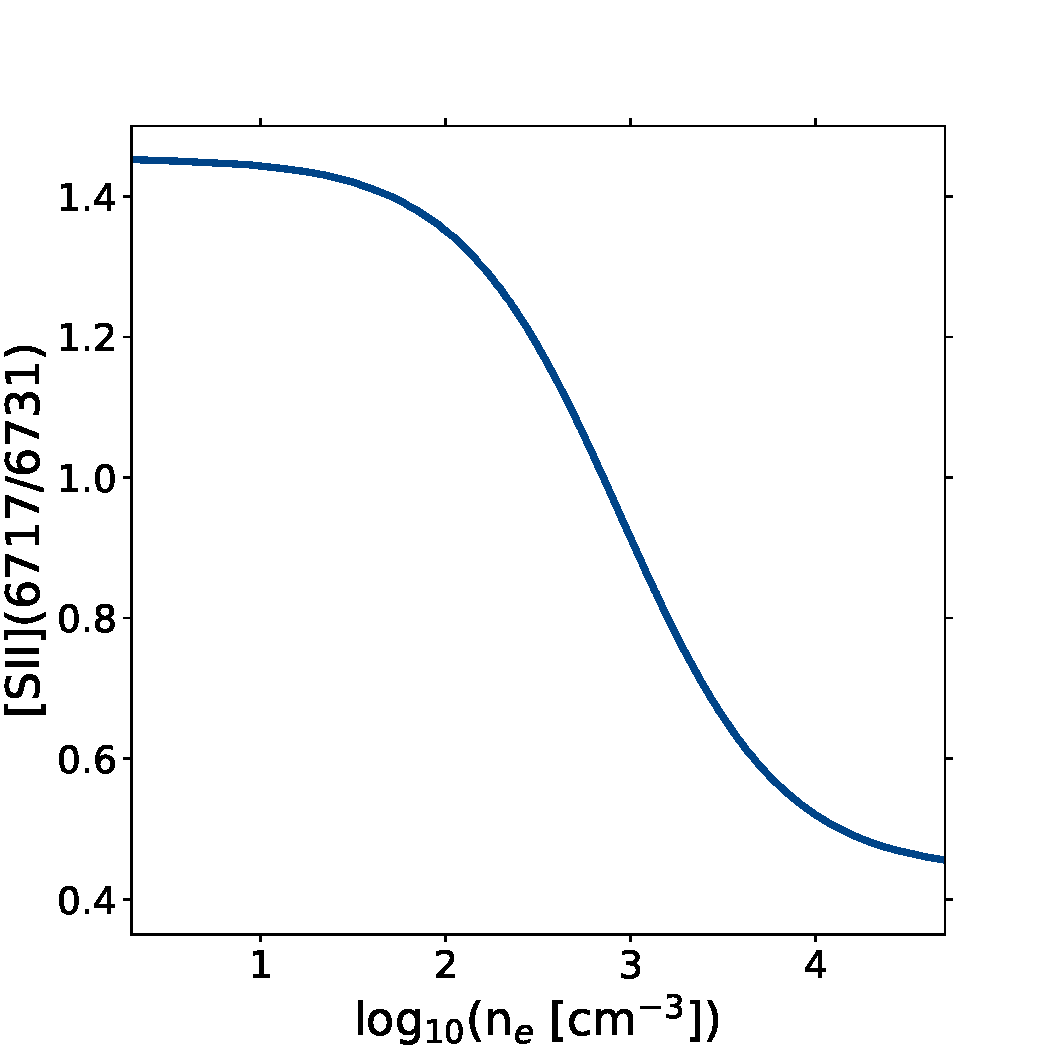
\includegraphics[width=0.7\linewidth]{figures/introduction/sii_ratio.pdf}
    \caption[{Variation of the [SII](6717/6731) emission-line flux ratio with electron density.}]{Variation of the traditional [SII](6717/6731) emission-line flux ratio with electron density, modelled with the \textsc{PyNeb} \textsc{Python} module \citep{Luridiana2015} for an ionised gas of temperature $T_e=10,000$\;K. This commonly-used density diagnostic is only sensitive to densities in the range 2.0\;\textless\;log$_{10}$($n_e$[cm$^{-3}$])\;\textless\;3.5: above and below these limits, the curve becomes increasingly asymptotic, and the values derived from this technique saturate.}
    \label{fig: introduction: outflows: energetics: warm_ionised: sii_ratio}
\end{figure}

However, these traditional, commonly-used ratios are only sensitive up to electron densities of $n_e\sim10^{3.5}$\;cm$^{-3}$ --- above this limit, both of the lines involved are collisionally suppressed, and the values of the ratios saturate. If, in reality, outflow densities are greater than $n_e\sim10^{3.5}$\;cm$^{-3}$, then this technique will underestimate true values. Crucially, since outflow masses (Equation\;\ref{eq: introduction: outflows: energetics: mout}), mass outflow rates (Equation\;\ref{eq: introduction: outflows: energetics: mout_rate}), kinetic powers (Equation\;\ref{eq: introduction: outflows: energetics: ekin}), and coupling efficiencies (Equation\;\ref{eq: introduction: outflows: introduction: e_f}) depend inversely on the electron density, this means that these derived properties would be overestimated. Therefore, it is notable that many studies which determine high outflow kinetic powers (i.e. $\epsilon_\mathrm{f}$\;\textgreater\;0.5\;per\;cent) also estimate or assume low electron densities ($n_e$\;\textless\;10$^{3.5}$\;cm$^{-3}$: e.g. \citealt{Kraemer2000II, Nesvadba2006, Harrison2014, Fiore2017}). Furthermore, the separation between the lines in the [SII] and [OII] doublets is small, and in the case of outflow kinematics --- in which line widths are typically intermediate-to-high (FWHM\;\textgreater\;500\;km\;s$^{-1}$) --- the lines are often blended. This introduces significant degeneracy in measuring the flux ratios, therefore preventing precise electron density determinations.

In the past decade, novel techniques of electron-density estimation have been developed which are sensitive to a wider range of values than the traditional [SII] and [OII] ratios. For example, \citet{Baron2019b} present a technique which uses the dimensionless ionisation parameter

\begin{equation}
    U=\frac{Q}{4{\pi}r^2cn_e},
    \label{eq: introduction: outflows: energetics: u}
\end{equation}

\noindent
where $Q$ is the number of ionising photons emitted by the AGN per second, and $r$ is the radial distance of the gas outflow from the AGN. In this method, the ionisation parameter is determined using emission-line ratios, $Q$ is derived from the bolometric luminosity of the AGN, and the outflow radial distance is determined from modelling the mid-infrared (MIR) spectral energy distribution (SED) of the AGN (see \citealt{Baron2019a}). Therefore, Equation\;\ref{eq: introduction: outflows: energetics: u} can be used to estimate the electron density, which \citet{Baron2019b} find to be in the range 3.0\;\textless\;log$_{10}$($n_e$\;[cm$^{-3}$])\;\textless\;6.2 for a sample of 234 Type\;2 AGN --- several orders of magnitude above the upper density limit of the traditional [SII] and [OII] ratios. Similarly, complex, multi-ionisation-component (i.e. multiple values of $U$) photoionisation modelling that utilises the measured fluxes of many emission lines has produced a wide range of electron densities when applied to outflows in nearby active galaxies (2.0\;\textless\;log$_{10}$($n_e$\;[cm$^{-3}$])\;\textless\;7.0: \citealt{Collins2009, Crenshaw2015, Revalski2021}; see also \citealt{Revalski2022}). 

Of particular note is a technique pioneered by \citet{Holt2011} using the [SII](4068 + 4076)/(6717 + 6731) and [OII](3726 + 3729)/(7319 + 7331) ratios, which involve the \textit{total} fluxes of the traditional [SII]$\lambda\lambda$6717,6731 and [OII]$\lambda\lambda$3726,3729 doublets in addition to the higher-critical-density transauroral \citep{Boyce1933} [SII]$\lambda\lambda$4068,4076 and [OII]$\lambda\lambda$7319,7331 doublets. By comparing the measured values of these ratios to predictions of photoionisation modelling, electron densities and reddenings can be derived simultaneously. Importantly, this technique is sensitive to a wider range of electron densities (2.0\;\textless\;log$_{10}$($n_e$\;[cm$^{-3}$])\;\textless\;5.5) than the traditional [SII](6717/6731) and [OII](3726/3729) ratios, but requires less-detailed observations (and is less computationally expensive) than the ionisation-parameter-based method presented by \citet{Baron2019b} and complex photoionisation modelling \citep{Collins2009, Crenshaw2015, Revalski2021}. Moreover, unlike the traditional [SII] and [OII] ratios, the transauroral-line method uses the \textit{total} fluxes of emission-line doublets instead of the fluxes of individual lines \textit{within} the doublets, obviating issues arising from degeneracy due to broad line widths.

In the past 13 years, the transauroral ratios have been used to measure gas densities in the range 3.0\;\textless\;log$_{10}$($n_e$\;[cm$^{-3}$])\;\textless\;5.5 in active galaxies of different types \citep{Holt2011, Rose2018, Santoro2018, Spence2018, RamosAlmeida2019, Santoro2020, Davies2020, Speranza2022}. These densities are up to two orders of magnitude higher than could be measured with the traditional ratios, and, correspondingly, modest outflow kinetic powers and coupling efficiencies have been derived ($\epsilon_\mathrm{f}$\;\textless\;0.5\;per\;cent). However, these studies have used spatially-unresolved observations, often with a single aperture covering the outflow region. Consequently, it has been argued that the transauroral lines are emitted by different clouds than those that emit other key diagnostic lines such as [OIII]$\lambda\lambda$4959,5007 and H$\beta$, and therefore that the derived densities are not representative of the outflowing gas (\citealt{Sun2017}; but see discussions in \citealt{Rose2018} and \citealt{Spence2018}). Since the outflow masses and kinetic powers resulting from transauroral-line-derived densities are much below those typically found for the warm ionised phase (and are potentially far below the values required by models of galaxy evolution), this situation needs to be investigated in detail to conclusively determine if the transauroral lines are valid tracers of outflowing gas.

\subsubsection{A low-surface-brightness, high-mass, warm ionised outflow component}

The techniques and studies described above for the warm ionised phase trace relatively dense ($n_e$\;\textgreater\;3.0\;cm$^{-3}$) gas in the central regions ($r$\;\textless\;2\;kpc) of active galaxies. While these studies find modest outflow masses and kinetic powers, it is possible that there also exists a tenuous ($n_e$\;\textless\;3.0\;cm$^{-3}$), low-surface-brightness, spatially-extended ($r$\;\textgreater\;5\;kpc) warm-ionised outflow component that the observations were not sensitive to. \citet{Spence2018} estimate that such a component could be ten times more massive than dense outflows in the centres of galaxies, despite only contributing 10\;per\;cent to the luminosities of key emission lines; this may form the powerful, galaxy-wide component of the outflows invoked by models of AGN in galaxy evolution \citep{DiMatteo2005,Springel2005,Schaye2015}. Therefore, deep, spatially-resolved, galaxy-scale studies of active galaxies with known small-scale ($r$\;\textless\;2\;kpc) outflows need to be performed in order to identify any potential spatially-extended, low-surface brightness counterparts.

\subsection{Outflow kinematics and geometry}
\label{section: introduction: outflows: kinematics_and_geometry}

\subsubsection{Outflow kinematics}
\label{section: introduction: outflows: kinematics_and_geometry: kinematics}

Determining accurate outflow kinematics is crucial, as the derived mass outflow rates (Equation\;\ref{eq: introduction: outflows: energetics: mout_rate}) and kinetic powers (Equation\;\ref{eq: introduction: outflows: energetics: ekin}) have square and cubic dependencies on velocity shifts (and dispersions), respectively. Kinematics are often derived in spectroscopic studies of AGN-driven outflows: as noted by \citet{Seyfert1943}, the line widths seen in the NLRs of nearby active galaxies are readily explainable by clouds of different velocities causing the Doppler-shifting of emission lines. In modern observational studies, prominent emission lines are used to determine kinematics --- perhaps the most commonly used is the [OIII]$\lambda\lambda$4959,5007 doublet, which is bright in typical AGN spectra, does not present broad wings from the BLR (Section\;\ref{section: introduction: historical_context: nlr_studies: unified scheme}) and, with the exception of extreme cases, is not blended with other emission lines. 

For a static cloud in a narrow line region, the dominant line-broadening effect would be Doppler motions of gas moving with a Maxwellian distribution of velocities, which is described by a Gaussian profile. Therefore, it is generally assumed that individual velocity components of a given emission-line profile follow a Gaussian distribution of wavelengths (or velocities). Consequently, many studies fit one or more Gaussian profiles (accounting for different velocity components) to outflow emission-line profiles to model the kinematics of the gas (e.g. \citealt{VillarMartin1999, Crenshaw2000_N1068, Das2005, Holt2011, Mullaney2013, Rose2018, Tadhunter2019}) --- often, the wavelength difference between the mean of a Gaussian component and the rest wavelength of the line is used to calculate velocity shift ($v$), and the width of the Gaussian component (either $\sigma$ or FWHM) is taken as a measure of the distribution of velocities within the cloud.

However, there are challenges to robustly interpreting outflow line profiles in terms of kinematics, mainly regarding projection effects: broad, complex line profiles may be produced by an ensemble of clouds with a large internal velocity dispersion, or by a system of clouds that is unresolved to the observer and has a small local velocity dispersion, and for which the clouds are flowing with a wide range of angles relative to the observer's line of sight (LOS). In terms of kinematics, complex line profiles therefore present a degeneracy: both of the described cases could give rise to an identical line profile, but the derived outflow velocities will change significantly depending on the assumed scenario. In an attempt to break this degeneracy, some studies use non-parametric approaches to de-project outflow kinematics. An example of this is percentile velocities, which involve measuring the velocity that contains a certain percentage of the total line flux under the assumption that the outflow velocity is the same in all directions (and that the local velocity dispersion is small), and therefore the far wings of line profiles (the maximum projected velocities) represent clouds moving along the line of sight (e.g. \citealt{CanoDiaz2012, Harrison2014, Rose2018}). In this approach, a velocity that contains 90\;per\;cent of the line flux would be represented by $v_{90}$. Similarly, some studies define non-parametric line widths based on the difference between two percentile velocities, for example $W_{80}=v_{90}-v_{10}$ (e.g. \citealt{Harrison2014, Venturi2021}). An example of these non-parametric approaches to measuring outflow kinematics is shown for a mock emission-line profile in Figure\;\ref{fig: introduction: outflows: kinematics: hbeta_v05_v95_w90}.

\begin{figure}[!t]
    \centering
    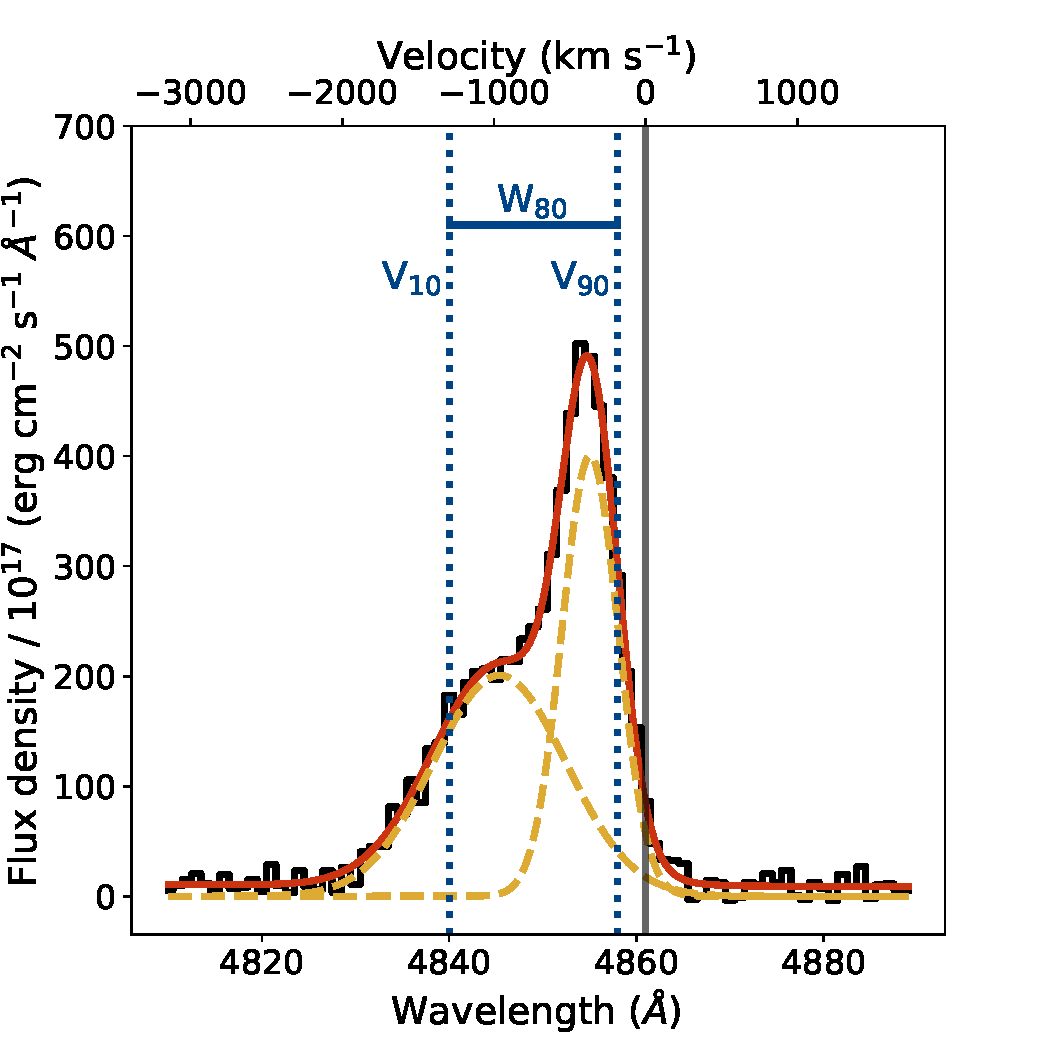
\includegraphics[width=0.7\linewidth]{figures/introduction/hbeta_v10_v90_w80.pdf}
    \caption[Examples of non-parametric percentile velocity shifts and widths for a simulated H$\beta$ line.]{Examples of non-parametric percentile velocity shifts ($v_\mathrm{10}$, $v_\mathrm{90}$: vertical dotted blue lines) and width ($W_\mathrm{80}$) for a simulated H$\beta$ line profile. The black line shows the simulated H$\beta$ emission, the solid red line shows the total fit, the dashed orange lines show the two individual Gaussian components required to fit the line profile, and the vertical solid grey line shows the rest wavelength of H$\beta$.}
    \label{fig: introduction: outflows: kinematics: hbeta_v05_v95_w90}
\end{figure}

The ideal approach to account for projection effects (and therefore determining robust kinematics) would be detailed modelling of NLR kinematics. For several nearby Seyfert galaxies, this has been done by fitting biconical, radial outflow models to kinematics derived from high-spatial-resolution HST spectra \citep{Crenshaw2000_N1068, Crenshaw2000_N4151, Das2005, Das2006, Das2007, Revalski2021}. However, such an approach requires detailed, spatially-resolved observations (and so is restricted to bright, nearby galaxies), is time-expensive, and relies on assumptions regarding outflow acceleration mechanisms, which themselves are not clear. Therefore, care must be taken when deciding how to measure outflow kinematics, and the method used should be considered when making physical interpretations based on derived outflow kinematics and energetics.

\subsubsection{Outflow spatial extents}
\label{section: introduction: outflows: kinematics_and_geometry: spatial_extents}

Models of galaxy evolution predict outflows that extend to galaxy-wide scales ($r$\;\textgreater\;5\;kpc: e.g. \citealt{Silk1998, DiMatteo2005, King2010, Curtis2016, Costa2018}). In contradiction to this, studies of nearby active galaxies that use long-slit spectroscopic observations with a technique called spectroastrometry --- which involves measuring the spatial centroid position of an emission line as a function of velocity along the slit \citep{Bailey1998} --- have found that warm-ionised outflows extend up to a few kiloparsecs (at maximum) from the central AGN \citep{Carniani2015, Spence2016, VillarMartin2016, Santoro2018, Santoro2020}, in agreement with the results of direct HST imaging \citep{Fischer2018, Tadhunter2018} and spectroscopy \citep{Das2005, Das2006, Das2007, Tadhunter2019}. In contrast, some optical integral field unit (IFU) studies have found outflows to be galaxy-wide \citep{Fu2009, Westmoquette2012, Liu2013, Harrison2014, Wylezalek2017}; since the observations used in these studies are ground-based, it has been suggested that the beam-smearing effects of atmospheric seeing artificially spread compact outflow emission from the central regions across the IFU field of view. This may have contributed to --- or been entirely responsible for --- the observed galaxy-wide outflow extents. Furthermore, \citet{Husemann2016} demonstrated that failure to account for beam smearing can result in overestimation of outflow kinetic powers by up to two orders of magnitude. Clearly, this situation needs to be investigated in detail, principally to determine the potential impact that atmospheric seeing can have on determinations of outflow spatial extents.

\subsection{Comparisons to models of galaxy evolution}
\label{section: introduction: outflows: comparisons_to_models}

In addition to the described uncertainties involved in calculating observationally-derived outflow kinetic powers, it is not clear if direct comparisons to the requirements of theoretical models of galaxy evolution are valid, or if interpretations drawn from such comparisons are robust. In this context, I highlight that, despite many observational studies attempting to verify models by comparing measured coupling efficiencies to those used in models, this parameter is not a \textit{predicted} quantity in such models: it is a free parameter that is set to reproduce the normalisation of the empirical SMBH-bulge scaling relations and properties of the local galaxy population.

Moreover, the AGN-feedback models used in cosmological simulations are not spatially resolved. One problem this can produce is numerical overcooling, which may be compensated for by increasing the required fraction of SMBH accretion power that is coupled to the ISM, potentially by orders of magnitude \citep{Weinberger2017} --- models that attempt to overcome this problem require a wide range of coupling efficiencies (0.04--30\;per\;cent: \citealt{Booth2009, Choi2012}). In addition, outflows may radiate a significant fraction of their energy post-acceleration, or decelerate under gravity, meaning that observationally-derived coupling efficiencies may be significantly lower than would be measured immediately after the outflow was launched. Furthermore, given that typical outflow dynamical timescales ($\sim$1--10\;Myr) may be similar to those of AGN cycles ($\sim$10--100\;Myr, although possibly much shorter in some cases: see \citealt{Morganti2017} for a review), it is unclear whether or not a given observed outflow was launched during the current epoch of AGN activity (the bolometric luminosity of which is used in coupling efficiency calculations). As argued by \citet{Harrison2018}, based on these arguments, it is not necessarily expected that coupling efficiency values required by models correspond to the measured ratio of outflow kinetic power to AGN bolometric luminosity, as is often assumed in observational outflow studies.

Therefore, direct comparisons of specific coupling efficiency values should be done with caution. Alternatively, \textit{qualitatively} comparing outflow properties derived from detailed observations to those predicted by tailored simulations of outflows in different object types may be an insightful (and perhaps complementary) approach. Detailed observational studies can also be used to inform the physics of the tailored models and the feedback prescriptions of cosmological simulations.


\subsection{Outflow acceleration mechanisms}
\label{section: introduction: outflows: acceleration_mechanisms}

A major barrier to robust comparisons of observations to theoretical models is that it is not clear how outflows are accelerated. AGN can launch outflows in two general ways: via radiation pressure from accretion disks, or via shocks induced in the ISM by jets. However, in many cases, both of these mechanisms can explain observed properties of the NLRs of local active galaxies, such as kinematics, spatial alignments between ionised gas and radio structures, and gas conditions \citep{Ulvestad1981, Wilson1985, Whittle1988, Cecil1990, Capetti1995a, Capetti1995b, Axon1998, Crenshaw2000_N1068, Crenshaw2000_N4151, Das2005, Das2006, Mukherjee2016, Mukherjee2018, Meena2021}. Furthermore, it is feasible that \textit{both} mechanisms could be present in a given galaxy, with their relative contributions to outflow acceleration and NLR ionisation/excitation being unclear.

\subsubsection{Radiatively-driven outflows}
\label{section: introduction: outflows: accleration_mechanisms: radiation}

The high luminosities produced by AGN accretion disks may impart significant radiation pressure on surrounding gas \citep{Castor1975, Abbott1982}, accelerating it via line-driving (bound-bound), continuum-opacity-driving (bound-free), and Thompson scattering (free-free) \citep{Arav1994, Murray1995, Proga1998, Proga2000}. In addition, dust may increase the effectiveness of radiation pressure driving on NLR gas at larger radii (\textbf{i.e. where it is not vapourised by radiation}; \citealt{Dopita2002, Fabian2006}). It has been proposed that these mechanisms can accelerate gas clouds in active galaxies to observed outflow velocities (up to several thousand kilometres per second; \citealt{Crenshaw2000_N1068, Crenshaw2000_N4151, King2003, Das2005, Das2006, Hopkins2010, King2010, MullerSanchez2011, Meena2021}). 

Two main variations of radiative driving are often invoked to explain observed NLR kinematics: radiation-driven winds launched close to the accretion disk that shock and accelerate the ISM on larger scales (e.g. \citealt{Elvis2000, Proga2000, King2003}), and radiation pressure directly accelerating colder NLR gas on kiloparsec-scales \textit{in situ} (e.g. \citealt{Das2007, Fischer2017, Revalski2018, Meena2021, Meena2023}). In an example of the former mechanism, \citet{Hopkins2010} propose that hot (4\;\textless\;log$_{10}(T [K])$\;\textless\;6), low-density ($n=1$--100\;cm$^{-3}$) gas close to the accretion disk ($r$\;\textless\;100\;pc) is radiatively accelerated to very high velocities ($v$\;\textgreater\;$10^4$\;km\;s\;$^{-1}$). As this high-velocity outflow impacts the colder, larger-scale ($r$\;\textgreater\;100\;pc) ISM, a series of shocks and dynamical instabilities cause it to mix with the colder gas, which produces an expansion in the direction perpendicular to the incident AGN radiation. The increased cross-section of the mixed cloud then leads to efficient, direct radiative driving. Very high-velocity nuclear winds such as those invoked in this model have been observed in the highly ionised phase (Table\;\ref{tab: introduction: outflows: energetics: multi-phase: outflow_phases}) with X-ray absorption lines \citep{Pounds2004, Lobban2011, Pounds2011, Tombesi2011}, and other studies making use of multi-wavelength observations have argued direct support for the importance of highly-ionised winds in driving larger-scale outflows \citep{Pounds2013, Feruglio2015}.

Tailored dynamical modelling that considers the balance of acceleration by radiation pressure and gravitational deceleration can reproduce the spatially-resolved outflow kinematics that are observed in the NLRs of some nearby active galaxies, lending support to radiation pressure being an important driving mechanism in these objects (\citealt{Crenshaw2000_N1068, Crenshaw2000_N4151, Das2005, Fischer2017, Revalski2018, Meena2021}). However, this requires high spatial- and spectral-resolution observations, and hence is limited to bright, nearby objects. Also, while this formalism can broadly explain the observed kinematics, in some cases, acceleration via shocks produced by jet-ISM interactions may be required \citep{Das2006, Das2007, Meena2023}. Furthermore, for several of the objects modelled in this way (e.g. NGC\;1068 and NGC\;4151), jet-ISM interactions alone may be able to explain observed spatial coincidence between radio structures and extreme NLR kinematics \citep{Capetti1995a, Capetti1995b, Axon1998, Das2006, May2017, May2020}, leaving the dominant acceleration mechanism unclear.

\begin{figure}[!t]
    \centering
    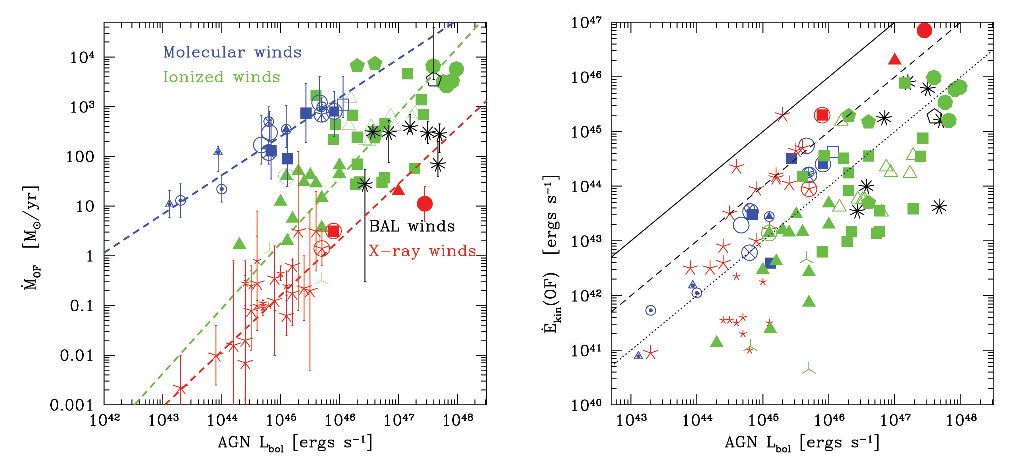
\includegraphics[width=\linewidth]{figures/introduction/fiore2017_mout_ekin_lbol.pdf}
    \caption[Observed multi-phase outflow scaling relations between outflow energetics and host AGN bolometric luminosity, as presented by \citet{Fiore2017}.]{Scaling relations between observed multi-phase outflow energetics (mass outflow rate: left; kinetic power: right) and AGN bolometric luminosity, produced by \citet{Fiore2017}. The red and black markers represent the energetics of highly-ionised X-ray and BAL (Broad Absorption Line; see review in \citealt{Gibson2009}) winds, green markers show energetics for warm-ionised outflows, and blue markers show the energetics of cold-molecular outflows. \textit{Image credit: \citet{Fiore2017}}.}
    \label{fig: introduction: outflows: acceleration_mechanisms: fiore2017_mout_ekin_lbol}
\end{figure}

Additional support for radiatively-driven outflows being common in active galaxies may be provided by statistical studies of a large number of objects. In particular, \citet{Fiore2017} collated observationally-derived mass outflow rates and kinetic powers for outflows and winds in the highly ionised, warm ionised, and cold molecular phases, and found scaling relations between these properties and AGN bolometric luminosity (Figure\;\ref{fig: introduction: outflows: acceleration_mechanisms: fiore2017_mout_ekin_lbol}). These relations may indicate that outflows in active galaxies are predominantly radiatively driven. However, it is unclear how observed mass outflow rates and kinetic powers of outflows driven by shocks from jet-ISM interactions would be expected to scale with bolometric luminosity. Furthermore, the uncertainties involved in deriving outflow energetics (Section\;\ref{section: introduction: outflows: energetics}) were not fully accounted for in producing these relations.

\subsubsection{Jet-driven outflows}
\label{section: introduction: outflows: accleration_mechanisms: jet_driven_outflows}

Feedback from AGN jets is commonly thought of in the context of powerful jets that extend far beyond the extents of host galaxies, such as those seen in Cygnus\;A \citep{Blandford1974, Carilli1991} and M87 \citep{Junor1999, Keiichi2012}. These jets reach the intergalactic or intracluster medium (IGM; ICM) and maintain the high temperatures and highly ionised states of halo gas, thus preventing catastrophic cooling and accretion to galaxy centres \citep{Binney1995, Soker2001, Best2006, McNamara2007, Gaspari2013}. On galaxy scales, these high-power jets are thought to pierce through the ISM without having a major impact or driving significant outflows (\citealt{Mukherjee2016}; see also \citealt{Scheuer1982, Hardee1990}). However, in the past two decades, theoretical work has demonstrated that lower-power jets ($P_\mathrm{jet}$\;\textless\;$10^{45}$\;erg\;s$^{-1}$) may instead provide an important source of feedback on galactic scales, as they are confined to the host galaxy medium for a longer time and hence affect a larger volume of the ISM (Figure\;\ref{fig: introduction: outflows: acceleration_mechanisms: mukherjee2016_high_low_power_jets}: \citealt{Mukherjee2016}; see also \citealt{Sutherland2007, Gaibler2011, Wagner2011, Mukherjee2016, Mukherjee2018}). In this scenario, the jets drive significant shocks into the ISM, heating and accelerating the gas and dissociating molecules. Modelling of jet-ISM interactions that includes both shock-ionisation induced by jets and photoionisation produced by AGN accretion disks predicts that the modelled ISM is predominantly shock-ionised \textbf{\citep{Meenakshi2022a}}, however, this has not been directly observationally verified.


\begin{figure}
    \centering
    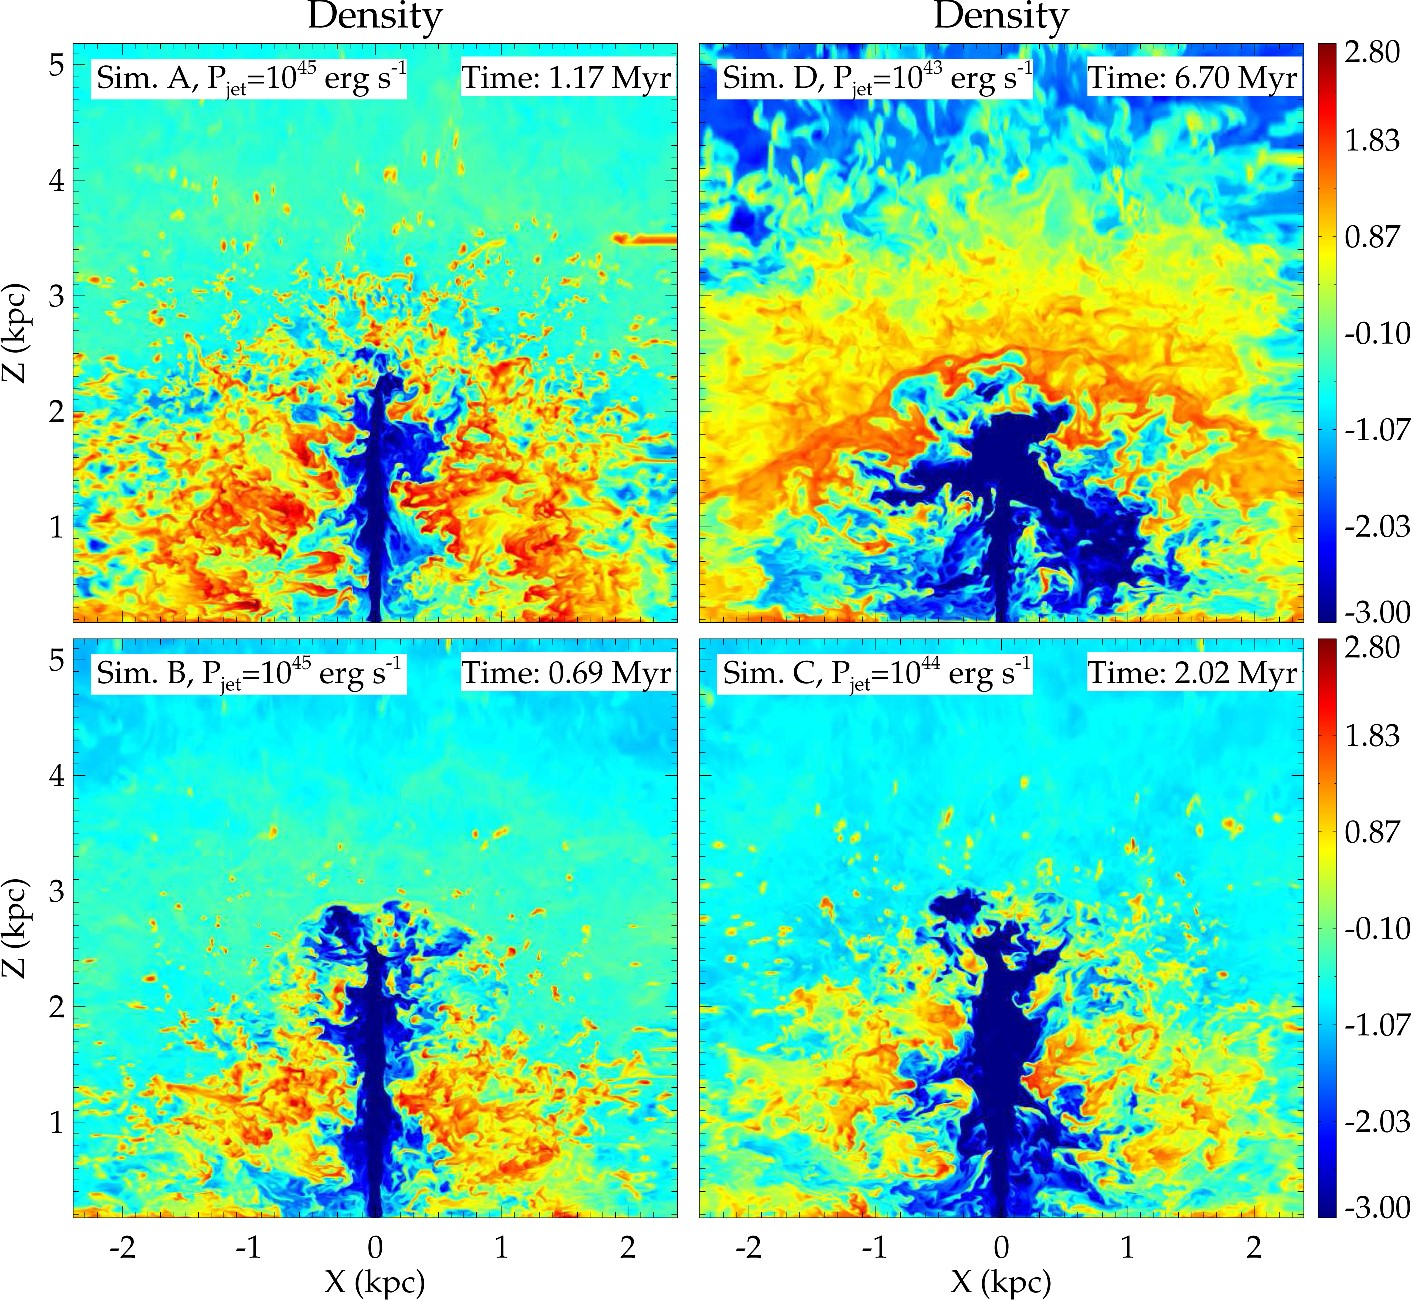
\includegraphics[width=\linewidth]{figures/introduction/mukherjee2016_high_low_power_jets.jpeg}
    \caption[Snapshots of hydrodynamic simulations by \citet{Mukherjee2016} of a higher- and lower-power jet propagating through an ISM.]{\textbf{Gas density [cm$^{-3}$] in a two-dimensional plane for hydrodynamic simulations of jets of different powers ($P_\mathrm{jet}=10^{45}$\;erg\;s$^{-1}$: left panels; $P_\mathrm{jet}=10^{44}$\;erg\;s$^{-1}$: bottom-right panel; $P_\mathrm{jet}=10^{43}$\;erg\;s$^{-1}$: top-right panel) propagating through the ISM at different times. For the highest-power-jet case, the simulation in the top-left panel (`Sim. A') considers an ISM that is twice as dense as the ISM considered in `Sim. B' (bottom-left panel). In these models, the higher-power jets pierce through the ISM and escape confinement quickly, launching modest-mass outflows, while the lower-power jets remain confined for a longer time, cause more disturbance, and launch higher-mass outflows. \textit{Image credit: \citet{Mukherjee2016}}.}}
    \label{fig: introduction: outflows: acceleration_mechanisms: mukherjee2016_high_low_power_jets}
\end{figure}

In addition to early outflow studies that found relations between disturbed NLR kinematics and radio structures (e.g. \citealt{Wilson1985, Whittle1988}), detailed observational studies have provided further evidence that jets drive outflows on galactic scales (e.g. \citealt{Morganti1998, Morganti2007, Nesvadba2008, Rosario2010a, Rosario2010b, Rosario2010c, Morganti2013_4c1250, Tadhunter2014, Mahony2016, May2017, Audibert2019, May2020, Venturi2021}). Of particular note are hydrodynamical simulations of AGN with low-power jets that can reproduce outflow properties derived from observational studies \citep{Morganti2015, Mukherjee2018, Audibert2023}.

In this context, it is interesting that a statistical study of a large sample of local ($z$\;\textless\;0.4), optically-selected AGN by \citet{Mullaney2013} found the broadest [OIII] emission-line profiles (indicative of more-prominent outflows) in objects of intermediate radio luminosity (23\;\textless\;log$_{10}$($L_\mathrm{1.4\;GHz}$[W\;Hz$^{-1}$])\;\textless\;25). Combined with the correlation between 1.4\;GHz luminosity and [OIII] line width previously found for Seyfert galaxies by \citet{Whittle1992c}, and the increased [OIII] line widths seen at the locations of prominent radio knots in the NLRs of Seyfert galaxies \citep{Whittle1988}, there is now considerable evidence that jets are an important outflow acceleration mechanism.

\subsubsection{Ionisation and excitation mechanisms as probes of acceleration}
\label{section: introduction: outflows: accleration_mechanisms: ionisation_and_excitation_mechanisms}

It is commonly assumed that different outflow acceleration mechanisms correspond to distinct gas ionisation or excitation mechanisms. For example, gas that has been directly radiatively-accelerated \textit{in situ} will have been subject to a significant flux of photo-radiation, therefore it is perhaps likely that at least the face of the cloud will be photoionised by the AGN. Conversely, material passing through a shock (driven into the ISM either by a fast nuclear wind or a jet) will be accelerated and heated to the hot ionised phase ($T$\;\textgreater\;$10^6$\;K), after which it will eventually cool to the warm ionised phase ($T\sim10,000$\;K) in which it can be observed with optical emission lines. Shock and photo-ionisation/excitation are expected to induce distinct physical conditions in the gas, for example in ionisation state and temperature \citep{Fosbury1978, Binette1996, VillarMartin1999}; these conditions can be probed by a range of flux ratios of emission lines arising from species of different ionisation/excitation potentials, and the emissivities of which are dependent on gas conditions such as temperature and density. Therefore, it is common practice to produce diagnostic diagrams in which two (or more) emission-line ratios are plotted to define distinct regions of different gas conditions (and hence ionisation mechanisms) to probe this.

The most commonly used diagnostic diagrams are those first presented by \citet{Baldwin1981} \textbf{and \citet{Veilleux1987} for the warm ionised phase}, referred to as BPT diagrams: the lines involved in these diagrams ([OIII]$\lambda5007$, H$\alpha$, H$\beta$, [NII]$\lambda$6584, [OI]$\lambda$6300, [SII]$\lambda\lambda$6717,6731) are bright in typical AGN optical spectra. By plotting the line ratios of known objects (e.g. star-forming regions, Seyfert galaxies, and LINERs\footnote{LINERs are a classification of galactic nuclei that display strong low-ionisation lines (such as [OI], [OII], [NII], and [SII]) in their spectra \citep{Heckman1980}}) on these diagrams, empirical regions are defined (see \citealt{Kewley2006}). Typically, it is thought that if an object has line ratios consistent with one of these regions, the dominant ionisation mechanism will correspond to that which is known for the object(s) from which the region was defined (commonly assumed to be photoionisation for the Seyfert/AGN region, and shocks for the LINER region). However, despite the BPT diagrams being used to distinguish between photoionisation and shock-ionisation in active galaxies (e.g. \citealt{Mingozzi2019, Venturi2021, Venturi2023, Revalski2021}), ionisation modelling shows that the regions of photo- and shock-ionisation overlap considerably (Figure\;\ref{fig: introduction: outflows: acceleration_mechanisms: bpt_diagram_photo_shock_ionisation}; \citealt{Dopita1995, Dopita1996, Allen2008, Ji2020}), preventing robust determinations of ionisation mechanisms for the warm ionised phase. 

\begin{figure}
    \centering
    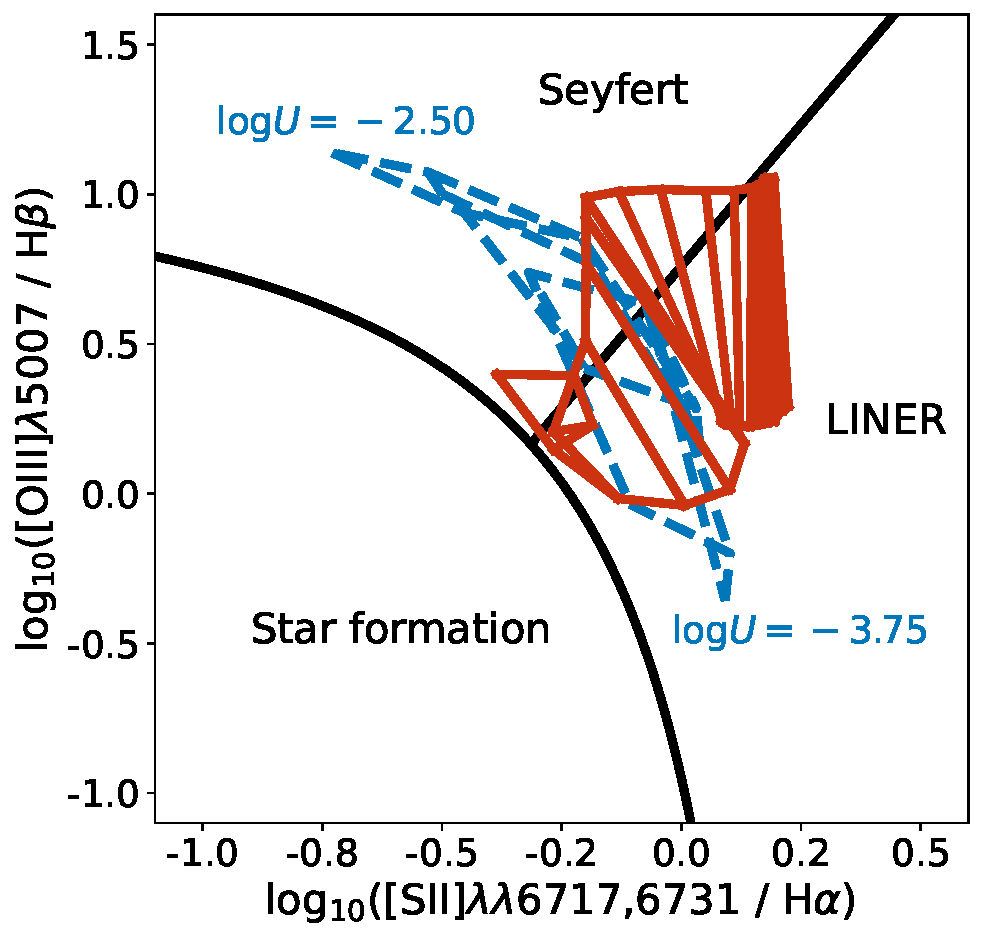
\includegraphics[width=0.75\linewidth]{figures/introduction/bpt_diagram_photo_shock_ionisation.pdf}
    \caption[{[SII]/H$\alpha$ vs [OIII]/H$\beta$ BPT \citep{Baldwin1981, Kewley2006} diagram with shock and photoionisation modelling.}]{[SII]/H$\alpha$ vs [OIII]/H$\beta$ BPT diagram \citep{Baldwin1981}, showing three empirically-defined regions \citep{Kewley2006} for Seyfert nuclei, star-forming regions, and LINERs, in addition to predictions of photoionisation (dashed blue grid) and \textbf{pure shock-ionisation (solid red grid) modelling}, which overlap significantly at the boundary between the Seyfert and LINER regions. The photoionisation models were generated using the \textsc{Cloudy} code (version C17.02: \citealt{Ferland2017}) for a radiation-bounded gas with varying ionisation parameter ($-3.75$\;\textless\;log$U$\;\textless\;$-2.50$; labelled) and electron density ($n_e=10^2,10^3,10^4$\;cm$^{-3}$), while the shock models are those generated using the \textsc{Mappings III} code by \citet{Allen2008} for shock velocities in the range 200\;\textless\;$v_\mathrm{shock}$\;\textless\;1000\;km\;s$^{-1}$ and magnetic parameters of $B/\sqrt{n}=2,10$\;$\mu$G\;cm$^{3/2}$.}
    \label{fig: introduction: outflows: acceleration_mechanisms: bpt_diagram_photo_shock_ionisation}
\end{figure}

To provide further information about the conditions of the warm-ionised gas, and to better discriminate between photo- and shock-ionisation, \citet{VillarMartin1999} created a diagnostic diagram plotting the [OIII](5007/4363) ratio against the He\;II$\lambda$4686/H$\beta$ ratio. The former ratio is dependent on the electron temperature of the emitting gas (shocked gas is expected to have higher temperatures: \citealt{Fosbury1978}), while the latter probes the presence of matter-bounded clouds, which may have similar temperatures to shocked gas \citep{Binette1996}. Therefore, the regions of photo- and shock-ionisation are more cleanly separated than in the typical BPT diagnostics. However, this diagram still only traces a single phase --- the warm-ionised gas.

Near-infrared (NIR) studies have revealed relations between emission-line flux ratios that may be powerful ionisation/excitation diagnostics of the warm ionised \textit{and} warm molecular phases. \citet{Larkin1998} first discovered a correlation between the NIR [FeII]$\lambda$12567/Pa$\beta$ and H$_2$(1--0)S(1)\;2.212\;$\mu$m/Br$\gamma$ ratios in LINERs, with higher values being associated with objects with known shocks. This correlation was subsequently confirmed, and empirical limits for different regions were refined using samples of star-forming galaxies (SFGs), LINERs, luminous infrared galaxies (LIRGs; L$_\mathrm{IR}$\;\textgreater\;$3.8\times10^{44}$\;erg\;s$^{-1}$: \citealt{Sanders1996}), and Seyfert galaxies, allowing the use of these ratios as a diagnostic diagram \citep{Rodriguez-Ardila2005, Riffel2013a, Colina2015, Riffel2021}. Since the H$_2$(1--0)S(1)\;2.212\;$\mu$m line arises from the warm molecular phase (Table\;\ref{tab: introduction: outflows: energetics: multi-phase: outflow_phases}), the H$_2$(1--0)S(1)\;2.212\;$\mu$m/Br$\gamma$ ratio axis of this diagram may be interpreted as tracing the relative excitation of the warm-molecular gas, with higher values associated with shock-excited gas. The physical interpretation for higher values of the [FeII]$\lambda$12567/Pa$\beta$ ratio is that iron is thought to be locked up in dust grains relatively easily: since dust grains are destroyed in shocks, iron is expected to be more abundant (and the [FeII]$\lambda$12567/Pa$\beta$ ratio therefore higher) post-shock. Support for this idea is provided by observed enhancements in the [FeII]$\lambda$12567/[PII]$\lambda$11886 ratio: phosphorus is less easily locked up in dust grains, and therefore it is notable that \citet{Riffel2013b} found enhanced values of [FeII]$\lambda$12567/[PII]$\lambda$11886 at the location of enhanced [FeII]$\lambda$12567/Pa$\beta$ along the radio axis of Seyfert\;1 galaxy Markarian (Mrk)\;79. This indicates that the [FeII]$\lambda$12567/Pa$\beta$ ratio is itself sensitive to the presence of shocks, which is further supported by an observed correlation between [FeII]$\lambda$12567/Pa$\beta$ and emission-line width (indicating that more-kinematically-disturbed gas has passed through a shock: \citealt{Riffel2021}).

\subsubsection{Photo- and shock-ionisation modelling}
\label{section: introduction: outflows: acceleration_mechanisms: modelling}

\textbf{Producing diagnostic diagrams with accurate regions for different ionisation mechanisms requires predicted emission-line-flux ratios from ionisation models of different types, principally photo- and shock-ionisation. However, there are important complexities and variations of these two main mechanisms that need to be carefully considered. For photoionisation models, there are two general ionised-cloud geometries: radiation-bounded and matter-bounded. In the former case, the ionised region of a given gas cloud (and therefore the ionisation front) is located well within the boundaries of the cloud itself, so that there exists a stratification consisting of fully-ionised, partially-ionised, and neutral-atomic gas within the cloud. For matter-bounded geometry, the outer boundary of the ionised region is the physical boundary of the cloud itself; the cloud is (almost) completely ionised. Therefore, compared to the radiation-bounded case, higher-ionisation emission lines are much stronger relative to lower-ionisation emission lines. Regarding shock-ionisation, modern models often consider two distinct ionisation sources: collisional ionisation as material passes through the shock, and the photoionisation of pre-shock gas by the approaching shock front (commonly referred to as the `precursor' ionisation component). The relative ionisation contribution of these two components is often unclear, and depends strongly on the properties of the ISM and the shock(s), hence it is common practice to produce distinct regions for pure-shock (referred to throughout this thesis as solely `shock') and precursor ionisation.}

\textbf{For gas densities that are typical for the NLR ($n\ll10^{10}$\;cm$^{-3}$), the photoionisation code \textsc{CLOUDY} \citep{Ferland2017} can readily produce radiation-bounded models that predict accurate line ratios for a range of gas and photoionising-source properties. However, generating photoionisation models with a mix of matter- and radiation-bounded clouds (required to determine relative contributions to line fluxes) with \textsc{CLOUDY} is complex --- a good supplement is to use the photoionisation models presented by \citet{Binette1996}, which provide the predicted fluxes of many key diagnostic lines for different relative fractions of radiation- and matter-bounded clouds. Used together, \textsc{CLOUDY} and the models of \citet{Binette1996} can produce diagnostic-diagram photoionisation regions for both photoionised-cloud geometries.}

\textbf{\citet{Allen2008} used the MAPPINGS III ionisation code to produce a suite of emission-line-flux predictions for both pure-shock and precursor ionisation for varying ISM and shock parameters. However, a major drawback of these models is that they only consider one spatial-dimension, which does not properly allow for additional thermal instabilities and potential secondary shocks (see discussion in \citealt{Allen2008}). While this could potentially affect simulated absolute line fluxes, the predictions of these models are still sufficiently accurate for placing the regions of expected shock-ionisation on diagnostic diagrams.}

\textbf{In general, a major problem with using photo- and shock-ionisation models to predict line ratios for the use in diagnostic diagrams is that the predicted ratios depend strongly on the properties of the ISM (e.g. gas densities and metallicities), photoionising sources (ionisation parameters, spectral indicies), and shocks (e.g. shock speeds and magnetic fields). Therefore, constraining these parameters where possible is essential, either via direct estimation using other methods (e.g. ionisation parameters from the technique presented by \citealt{Baron2019a} and electron densities from the transauroral-line ratio technique of \citealt{Holt2011}) or assuming a range of reasonable values (such as magnetic parameters that are characteristic of the ISM: \citealt{Allen2008}; see Figure \ref{fig: introduction: outflows: acceleration_mechanisms: bpt_diagram_photo_shock_ionisation}).}

\subsubsection{Uncertainties regarding outflow acceleration mechanisms}
\label{section: introduction: outflows: accleration_mechanisms: conclusions}

Overall, AGN-driven-outflow acceleration mechanisms are poorly understood, and are a matter of significant debate: there are many contradictions and claims of different mechanisms being dominant, even for individual objects (e.g. for NGC\;1068: \citealt{Axon1998, Crenshaw2000_N1068, Das2005, Fischer2017, May2017,  Revalski2021, Meena2023}). Principally, this is because the relationship between acceleration mechanisms and outflow ionisation/excitation is not clear, nor is the connection between NLR gas properties and radio structures.

The kiloparsec-scale linear double or triple radio structures seen in Seyfert galaxies (e.g. Figure\;\ref{fig: introduction: historical_context: nlr_studies: wilson1982_ngc1068_15ghz}: \citealt{Wilson1982}; \citealt{Wilson1980, Pedlar1983, Pedlar1984, Ulvestad1984}) are likely tracing synchrotron emission produced by shocks or radio plasma \citep{Wilson1980, Ulvestad1984}. It is commonly argued that, based on the morphologies of these structures and the presence of small-scale radio knots close to the nucleus, these structures represent AGN jets propagating into the ISM (e.g. \citealt{Wilson1982, Stanghellini2005, Rosario2010b, Riffel2013b, Jarvis2019, Williams2017, Girdhar2022}). In contrast, other authors have argued that the synchrotron emission is produced by shocks that are induced when radiatively-driven winds (i.e. such as those invoked in modelling by \citealt{Hopkins2010}; see Section\;\ref{section: introduction: outflows: accleration_mechanisms: radiation}) impact the ISM, launching kpc-scale outflows in the process (\citealt{Fischer2019}; see also \citealt{Fischer2023}).

Regardless of the source of the shocks, it is not clear how well ionisation/excitation mechanisms correspond to radiative or shock-acceleration. While line ratios consistent with shock-ionisation/excitation indicate that the emitting material has passed through (and thus been accelerated by) a shock, photoionised gas does not necessarily imply radiative acceleration: it is possible that the material passed through a shock, cooled, and then was re-ionised by radiation from the AGN. 

Determining precise diagnostics of outflow acceleration, ionisation/excitation, and the links between these is therefore essential: simulations of different mechanisms are now able to predict specific outflow properties (e.g. \citealt{Richings2021, Meenakshi2022a, Meenakshi2022b}; see \citealt{Krause2023} for a review), allowing detailed observational studies to directly test their assumptions regarding the underlying physics. Moreover, a complete understanding of outflow acceleration is needed to inform the sub-grid\footnote{\textbf{Many cosmological simulations divide the three-dimensional volume that they consider into a grid of cells; the spatial size of the cells effectively sets the spatial resolution of the simulation. `Sub-grid' refers to processes in such simulations that take place on scales smaller than the cell size.}} physics of cosmological simulations, for which AGN feedback in the form of outflows is required to reproduce observed galaxy properties \citep{Schaye2015, Dubois2016, Dave2019, Zinger2020}.

\subsection{Taxonomy of AGN}
\label{section: introduction: outflows: taxonomy_of_agn}

Active galaxies of different types provide distinct, useful laboratories to investigate outflow properties and acceleration mechanisms. Here, I briefly summarise AGN classification (see \citealt{Netzer2015} and \citealt{Tadhunter2008, Tadhunter2016} for reviews) and define the types of galaxies and AGN that are considered in this thesis. 

\subsubsection{Optical classifications}
\label{section: introduction: outflows: taxonomy_of_agn: seyferts_and_quasars}

The term `Seyfert' galaxy was originally used to refer to nearby active galaxies with nuclei that showed optical spectral features characteristic of planetary nebulae, indicating high ionisation. As described in Section\;\ref{section: introduction: historical_context: early_studies}, the systematic study of these objects began with the seminal work of \citet{Seyfert1943}; subsequent studies often adopted various definitions for the term based on properties such as optical and radio luminosities \citep{Wilson1980}, emission-line ratios \citep{Baldwin1981}, and line widths \citep{Whittle1992a}. In this thesis, I define Seyfert galaxies\footnote{Some classical Seyfert galaxies --- notably NGC\;1068, which is considered in Chapter\;\ref{chapter: stis_seyferts} --- have bolometric luminosities that are close to (and potentially above) the limit used in this definition.} to be galaxies with nuclei that present line ratios that are consistent with the AGN/Seyfert regions of the BPT diagrams (to separate them from LINERs and star-forming/HII galaxies: \citealt{Baldwin1981, Kewley2006}), line widths of FWHM\;\textgreater\;200\;km\;s$^{-1}$, and have bolometric luminosities of $L_\mathrm{bol}$\;\textless\;10$^{45}$\;erg\;s$^{-1}$ (to distinguish them from quasars).

Although quasars were originally considered to be a distinct class of object (Section\;\ref{section: introduction: historical_context: radio_astronomy}), it is now accepted that they are intrinsically the same phenomenon as Seyfert galaxies, only with higher optical luminosities; there likely exists a continuous scale of bolometric luminosity between the two classes. Therefore, here I define quasars (QSOs) to be objects with the same properties as Seyfert galaxies, except with higher bolometric luminosities ($L_\mathrm{bol}$\;\textgreater\;10$^{45}$\;erg\;s$^{-1}$).

As discussed in Section\;\ref{section: introduction: historical_context: nlr_studies: unified scheme}, by the end of 1960s, it was appreciated that Seyfert galaxies present a dichotomy in the widths of their forbidden and permitted lines. Therefore, they were sub-classified into Seyfert\;1s, which present narrow (200\;\textless\;FWHM\;\textless\;1000\;km\;s$^{-1}$) forbidden lines and broad (FWHM\;\textgreater\;1000\;km\;s$^{-1}$) permitted lines, and Seyfert\;2s, which present narrow forbidden and permitted lines \citep{Khachikian1971}. With the recognition that Seyfert galaxies and quasars are likely the same phenomenon, these classifications were extended to quasars (QSO1s and QSO2s), and later generalised to all AGN (Type\;1 and Type\;2). In the unified scheme of AGN (Figure\;\ref{fig: introduction: historical_context: nlr_studies: unified_scheme}), Type\;1 and Type\;2 AGN of a given class are the same intrinsic phenomenon, only viewed along different lines of sight.

Seyfert galaxies and quasars --- as defined here --- provide different regimes for probing AGN feedback in the inner regions of galaxies ($r$\;\textless\;5\;kpc). Owing to their higher bolometric luminosities, quasars are perhaps expected to impart greater radiation pressure on NLR gas (and/or drive stronger radiatively-driven winds) than Seyfert galaxies, and therefore photoionisation and radiative outflow-acceleration may be dominant. In contrast, the lower bolometric luminosities of Seyfert galaxies may mean that potential optical tracers of jet-ISM interactions are not obscured by dominant photoionisation that results from the intense radiation of the central AGN, and, based on previous NLR studies (e.g. \citealt{Whittle1992a, Axon1998, Crenshaw2000_N1068, Das2007}), it may be expected that they are more likely to host a mixture of jet- and radiation-driven outflows.

Similar to the classification schemes for objects detected at optical wavelengths, the optical properties of radio galaxies (galaxies detected via their radio emission) are often separated into the Broad Line Radio Galaxy (BLRG; Type 1 AGN: \citealt{Osterbrock1976, Grandi1977}) and Narrow Line Radio Galaxy (NLRG; Type 2 AGN: \citealt{Costero1977}) subclasses. However, objects of these classifications (collectively known as Strong Line Radio Galaxies, or SLRGs: e.g. \citealt{RamosAlmeida2011}) form only a subset of the radio-galaxy population: a significant fraction of radio galaxies instead present weak optical emission lines (known as Weak Line Radio Galaxies, or WLRGs: \citealt{HineLongair1979, Best2012}). The SLRG and WLRG classes --- defined by the [OIII]$\lambda5007$ equivalent width (e.g. $\mathrm{EW}_\mathrm{[OIII]}$\;\textless\;10\;{\AA} for WLRGs: \citealt{Tadhunter1998}) --- have considerable (but not complete) overlap with the commonly-used classifications of High Excitation Radio Galaxies (HERGs: \citealt{Laing1994, Tadhunter1998, Best2012}; see discussion in \citealt{Tadhunter2016}) and Low Excitation Radio Galaxies (LERGs), respectively, which are defined based on measured emission-line ratios (e.g. \citealt{Buttiglione2010}).

Although not directly considered in this thesis, also of note is the LINER (Low Ionisation Nuclear Emission Region) classification \citep{Heckman1980}, comprising objects that display prominent low-ionisation lines (e.g. [OI], [OII], [NII], [SII]), but weak high-ionisation lines (e.g. [OIII]), in their spectra. It is not clear whether LINERs are a true class of AGN or if the observed ionisation is (at least in part) due to stellar radiation \citep{CidFernandes2011, Singh2013, Coldwell2018, Frederick2019}. As discussed earlier, emission-line widths and diagnostic diagrams making use of multiple emission-line ratios (such as the BPT diagnostics: e.g. Figure\;\ref{fig: introduction: outflows: acceleration_mechanisms: bpt_diagram_photo_shock_ionisation}) can be used to distinguish between bonafide AGN and non-AGN LINERs.


\subsubsection{Radio classifications}
\label{section: introduction: outflows: taxonomy_of_agn: css_and_gps_sources}

As a result of radio astronomy playing a prominent role in the development of AGN as an important field of modern astrophysics, there are also classification schemes based on object properties at radio frequencies (see \citealt{Tadhunter2016} for a comprehensive review). The earliest AGN detected and identified at radio wavelengths are luminous radio sources ($L_\mathrm{1.4\;GHz}$\;\textgreater\;$10^{25}$\;W\;Hz$^{-1}$), and often have radio structures that extend far beyond their host galaxies (e.g. $r_\mathrm{jet}\sim60$\;kpc for Cygnus\;A: \citealt{Carilli1991}); the most-commonly-used radio classifications are the Fanaroff-Riley classes \citep{Fanaroff1974}, which separate such radio morphologies into `edge-darkened' (FR\;I) and `edge-brightened' (FR\;II; e.g. Cygnus\;A).

However, there also exist classes of luminous radio AGN that present complex radio structures on sub-galactic scales, the most important of which are compact steep spectrum (CSS) and gigahertz peaked spectrum (GPS) sources  (see \citealt{ODea1998} and \citealt{ODea2021} for reviews). The radio structures of CSS sources typically have radial extents of $r$\;\textless\;15\;kpc and have steep ($\alpha$\;\textless\;$-0.5$)\footnote{Radio continua are typically characterised by spectral indices ($\alpha$), defined as $F_\mathrm{\nu}\propto\nu^\alpha$, where $F_\mathrm{\nu}$ is the monochromatic flux density at the frequency $\nu$.} radio spectra, while those of GPS sources are typically sub-kpc-scale and peak at gigahertz frequencies \citep{Kellermann1981, ODea1998, Callingham2015}. The morphologies of these sources are often double or triple, similar to those seen in classical Seyfert galaxies (Figure\;\ref{fig: introduction: historical_context: nlr_studies: wilson1982_ngc1068_15ghz}: \citealt{Wilson1982}) and in radio galaxies on larger scales (FRII), indicative of jets. The compactness of the radio structures of CSS/GPS sources may be explainable if their jets are young and/or are being confined by the dense ISM \citep{Bicknell1997, Stanghellini2005, ODea2021}, from which they eventually grow and subsequently evolve into larger-scale radio galaxies \citep{Stanghellini2005, Morganti2007, Kukreti2023}. This process would be expected to entail prominent jet-ISM interactions, and thus CSS/GPS sources host powerful outflows (e.g. \citealt{Holt2008, Holt2011, Santoro2020}).

\subsubsection{Ultra luminous infrared galaxies}
\label{section: introduction: outflows: taxonomy_of_agn: ulirgs}

Finally, although not strictly a class of AGN, ultra luminous infrared galaxies (ULIRGs) are an important class of galaxy for studies of AGN-driven outflows. These are defined as galaxies with infrared luminosities above 10$^{12}$ solar luminosities ($L_\mathrm{5-500\;\mu{m}}$\;\textgreater\;$3.8\times10^{45}$\;erg\;s$^{-1}$: \citealt{Sanders1996}). Almost all (\textgreater\;90\;per\;cent: \citealt{Veilleux2002}) ULIRGs show morphological evidence for strong tidal interactions, and so it is thought that they represent the peaks of gas-rich major mergers. Therefore, they are considered to be the most rapidly evolving galaxies in the local Universe, and thus represent the situation modelled in hydrodynamical simulations which predict AGN triggered in mergers that launch galaxy-wide outflows \citep{DiMatteo2005, Springel2005, Hopkins2008, Johansson2009}. Indeed, a significant fraction ($\sim$40--70\;per\;cent: \citealt{Kim1998, Veilleux2002, Nardini2010, AlonsoHerrero2012}) of ULIRGs host AGN. For these reasons, they are expected to host prominent outflows, which have been now observed in a range of gas phases (e.g. \citealt{Zaurin2013, Spence2018, Rose2018, Tadhunter2019, Lamperti2022}).

\section{Outstanding problems addressed by this thesis}
\label{section: introduction: outstanding problems}

Overall, while significant progress has been made in understanding AGN-driven outflows over the past twenty-five years, their true properties, natures, and role in galaxy evolution are still largely unclear. Key outstanding questions include the following. \\

\begin{itemize}
    \item Which outflow phase(s) is dominant in terms of mass and kinetic power, and how are the different phases physically linked?
    \item What are the true electron densities of the warm ionised outflow phase, and what is the impact on derived outflow kinetic powers?
    \item Are AGN-driven outflows truly galaxy-wide, as predicted by simulations of galaxy evolution?
    \item How are outflows accelerated by AGN, and what is the relationship between outflow excitation/ionisation mechanisms and acceleration mechanisms? \\
\end{itemize}

To address these important questions, in this thesis I present detailed studies of four nearby active galaxies, three of which are classified as Seyfert galaxies and the other a ULIRG/QSO/GPS source. The studies make use of deep, high-spatial-resolution, multi-wavelength observations that trace different gas phases --- in addition to developing and utilising precise outflow diagnostic techniques --- to robustly quantify outflow properties and interpret their impact on the host galaxies. The observations and analyses are presented in the chapters of this thesis as follows. \\

\begin{itemize}
    \item In Chapter\;\ref{chapter: xshooter_ic5063}, I present a study based on high-spatial-resolution, wide-wavelength-coverage long-slit VLT/Xshooter spectroscopy of the kpc-scale radio structure of the nearby Sey\;2 galaxy IC\;5063, which is known to host prominent jet-driven outflows. The principal aims of this analysis were to determine robust spatially-resolved electron densities using the transauroral-line method (for the first time), verify the use of this method in studies of AGN-driven outflows, and place the resulting precise warm-ionised outflow properties in a multi-phase context using the wealth of previous observations of this object, therefore allowing an investigation into the relative importance of the various outflow phases and the physical link(s) between them. The work presented in this chapter is based on the 1st first-author publication of my PhD \citep{Holden2023}.
    \item Extending this analysis to other nearby active galaxies, in Chapter\;\ref{chapter: stis_seyferts} I analyse HST/STIS spectroscopy of the inner few-hundred parsecs of the prototypical Seyfert galaxies NGC\;1068 and NGC\;4151. Using the transauroral-line technique, this data is used to measure spatially-resolved electron densities for these two objects, which are then compared to the results of previous detailed photoionisation modelling to further verify this method. Moreover, the high-spatial-resolution STIS observations allow for the ionisation conditions of the gas to be determined; combining this with information regarding the radio structures in the NLRs, the link between ionisation and acceleration mechanisms is investigated, permitting a detailed study into the launching mechanism of the outflows. This analysis and subsequent results were first presented in the 2nd first-author publication of my PhD \citep{HoldenTadhunter2023}.
    \item Chapter\;\ref{chapter: alma_f13451_1232} presents an ALMA CO(1--0) study of the cold-molecular gas in the inner few kiloparsecs of the primary nucleus of the ULIRG/QSO/GPS source F13451+1232, an object which directly represents the situation considered in models of galaxy evolution. While compact ($r$\;\textless\;100\;pc) outflows have been detected in this object in various phases previously, there has not yet been a robust detection of molecular outflows --- a potentially crucial phase. The ALMA CO(1--0) observations are used to search for molecular outflows, with the aim of completing the multi-phase information and thus allowing for the relative importance of the various phases to be established for an object of higher radio and bolometric luminosity than the Seyfert galaxies considered in prior chapters. Furthermore, the high spatial resolution of the ALMA observations allows for the spatial extents of molecular outflows to be determined (thus addressing a prediction of galaxy evolution models), and by combining them with archival VLBI observations, the outflow acceleration mechanism(s) are investigated. This chapter is based on the third 1st-author publication of my PhD \citep{Holden2024}.
    \item The techniques and analyses used in the previous three chapters are sensitive to relatively dense ($n_e$\;\textgreater\;$10^{3}$\;cm$^{-3}$) gas in the central kiloparsecs of galaxies. Therefore, to directly verify the true spatial extents of the warm ionised outflow phase, Chapter\;\ref{chapter: muse_f13451_1232} presents a VLT/MUSE IFU study of F13451+1232 on galaxy-scales ($r$\;\textgreater\;5\;kpc) --- an object which, according to models of galaxy evolution, would be expected to host prominent galaxy-wide outflows. Unlike previous, similar ground-based IFU studies of outflows in local AGN, the analysis of this chapter carefully accounts for the beam-smearing effects of atmospheric seeing, and quantifies its effect on key outflow properties including spatial extents, kinematics, mass outflow rates, and kinetic powers.
    \item Finally, in Chapter\;\ref{chapter: conclusions_and_future_work} I summarise the results of these chapters and present the conclusions of this thesis. Moreover, I discuss future work that can be undertaken in this field, in addition to important considerations that are required for further significant progress to be made in understanding the nature of AGN-driven outflows and their role in galaxy evolution.
\end{itemize}
